% !TEX root = ../main.tex
\chapter{多元函数微分学}

一元函数微分学只处理 $y=f(x)$ 这种一个因变量对应一个自变量的情况。我们把视野扩展到多个自变量，进入多元函数微分学。多元函数微分学主要研究“一对多”和“多对多”关系下的求导问题，核心思想与一元情形一脉相承，只是多了一些方向和维度的考量。

\section{多元函数初步}
和一元函数一样，我们需要先定义多元函数和它的相关概念，才能更好地研究多元函数本身和它的相关性质。不过本书主要讨论二元函数，对更多元的函数不作展开。

\subsection{空间中的点集与多元函数}

我们先回忆一下第一章中邻域的概念：$x_0$ 的 $\delta$ 邻域是数轴上以 $x_0$ 为中心、左右各延伸 $\delta$ 的一个开区间。也就是说，邻域在一元函数的时候，是一个一维的区域，那么，推广到二元函数，就是二维区域，更进一步的，推广到我们的三维空间，就能得到：

\begin{definition}{三维空间的邻域}{}
设 $P_0(x_0, y_0, z_0)$ 是空间中的一点，$\delta > 0$。称集合
\[
U(P_0, \delta) = \{ P \mid |PP_0| < \delta \} = \{ (x,y,z) \mid (x-x_0)^2 + (y-y_0)^2 + (z-z_0)^2 < \delta^2 \}
\]
为点 $P_0$ 的 $\delta$ \textbf{邻域}。它是一个以 $P_0$ 为球心、$\delta$ 为半径的\textbf{开球}。
\end{definition}

开球的意思是这个球不包含球面：

\begin{center}
  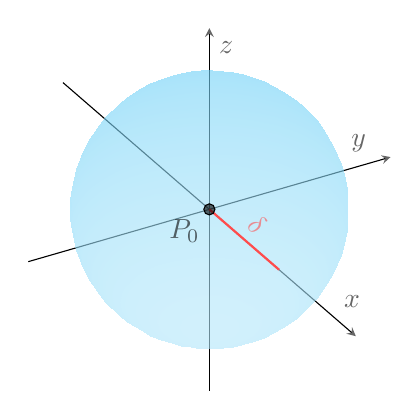
\begin{tikzpicture}
    % 设置三维视角
    \begin{axis}[
      scale=1.5,
      scale only axis=true,
      axis lines=center,       % 坐标轴过原点
      axis equal image,        % 三轴等比例
      xlabel={$x$}, ylabel={$y$}, zlabel={$z$},
      xmin=-3.5, xmax=3.5,
      ymin=-2.5, ymax=2.5,
      zmin=-2.5, zmax=2.5,
      view={60}{30},           % 视角，可调整
      ticks=none,              % 不显示刻度
      enlargelimits=0.1,
      domain=0:360,
      y domain=0:180,
      samples=40,              % 网格密度
      samples y=20,
      surf,                    % 曲面着色
      faceted color=cyan!30,   % 网格线颜色
      fill opacity=0.6,        % 透明度
      colormap={white}{color(0cm)=(cyan!30); color(1cm)=(cyan!60)} % 颜色映射
      ]
      
      % 绘制球面：半径为2，用球坐标 (x=r sinθ cosφ, y=r sinθ sinφ, z=r cosθ)
      \addplot3[surf, shader=interp, draw=blue!30, dashed, very thin]
               ({2*sin(y)*cos(x)},
                {2*sin(y)*sin(x)},
                {2*cos(y)});
                
      % 标记球心
      \addplot3[mark=*, mark size=2pt, color=black] coordinates {(0,0,0)}
          node[below left] {$P_0$};
      
      % 绘制半径线段（从球心到(2,0,0)）
      \addplot3[red!70, thick, no markers] coordinates {(0,0,0) (2,0,0)}
          node[midway, above, sloped] {$\delta$};
          
    \end{axis}
  \end{tikzpicture}
\end{center}

接下来我们要定义点集。类似的，一元函数的定义域是数轴上的一个区间，二元函数的定义域是平面上的一个区域，三元函数的定义域就是空间中的一个点集：

\begin{definition}{点集}{}
  由点构成的集合称为点集，记为 $E$。
\end{definition}

有了邻域和点集，我们可以描述点和点集之间的关系：

\begin{definition}{点和点集之间的关系}{}
设 $E$ 是空间中的一个点集，$P$ 是空间中的一点，定义：

\textbf{内点}：若存在 $\delta > 0$，使得 $U(P, \delta) \subseteq E$，则称 $P$ 是 $E$ 的\textbf{内点}。

\textbf{外点}：若存在 $\delta > 0$，使得 $U(P, \delta) \cap E = \varnothing$，则称 $P$ 是 $E$ 的\textbf{外点}。

\textbf{边界点}：若在 $P$ 的任意邻域内，既有 $E$ 中的点，又有不在 $E$ 中的点，则称 $P$ 是 $E$ 的\textbf{边界点}。
\end{definition}

简单来说，内点是“完全在里面的点”，外点是“完全在外面的点”，边界点是“踩在边界上的点”。比如开圆盘 $x^2+y^2 < 1$ 的内点是所有严格在圆内的点，边界点是圆周 $x^2+y^2=1$ 上的点。

有了这些概念，我们可以定义开集和闭集：

\begin{definition}{开集和闭集}{}
\textbf{开集}：若点集 $E$ 中的每一个点都是内点，则称 $E$ 为\textbf{开集}。

\textbf{闭集}：若点集 $E$ 的补集是开集，则称 $E$ 为\textbf{闭集}。
\end{definition}

例如，开球 $U(P_0, \delta)$ 是开集，包含球面的球是闭集。区间 $(a,b)$ 是开集，$[a,b]$ 是闭集，$[a,b)$ 既不开也不闭。这些和一元情形完全类似。

最后，我们还需要“连通”的概念。多元函数的定义域通常要求是连通的。直观地说，就是“一整块”，通常不能分成互不相交的几块。

\begin{definition}{连通}{}
  若\textbf{不存在}两个不相交的开集 $A$ 和 $B$，使得点集 $E \subseteq A \cup B$ 且 $E \cap A \neq \varnothing$，$E \cap B \neq \varnothing$，则称点集 $E$ 是\textbf{连通的}。
\end{definition}

\begin{center}
  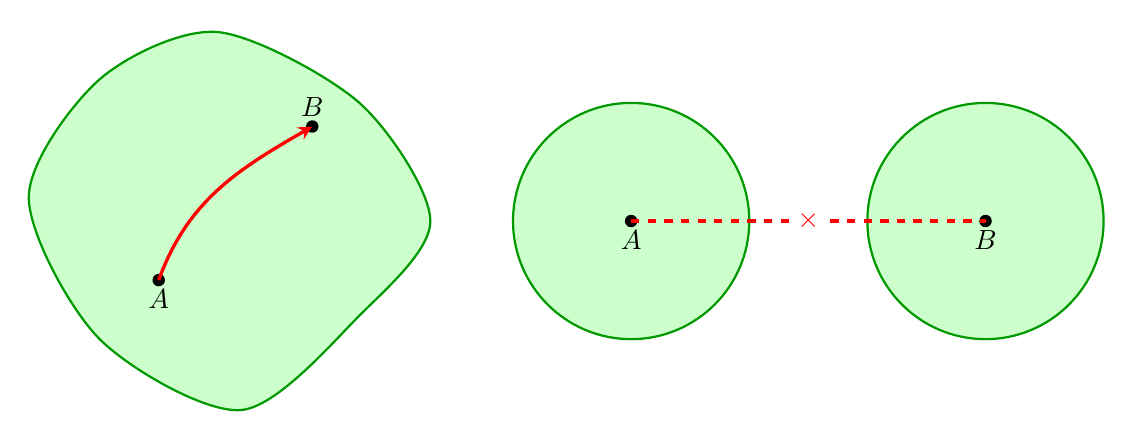
\begin{tikzpicture}[scale=1.5]
  
    % ========== 左：连通集 ==========
    \begin{scope}[local bounding box=left]
  
      % 画一个不规则但连通的区域（用光滑闭合曲线）
      \path[fill=green!20, draw=green!60!black, thick]
           plot[smooth cycle] coordinates {
               (0,0) (1.2,-0.6) (2.2,0.2) (2.8,1.0)
               (2.2,2.0) (1.0,2.6) (0.0,2.2) (-0.6,1.2)
           };
  
      % 区域内的两点 A 和 B
      \coordinate (A) at (0.5, 0.5);
      \coordinate (B) at (1.8, 1.8);
  
      \fill (A) circle[radius=1.5pt] node[below] {$A$};
      \fill (B) circle[radius=1.5pt] node[above] {$B$};
  
      % 红色实线表示能在区域内连接 A、B
      \draw[red, very thick, ->, >=stealth]
           (A) to[out=70, in=210] (B);
    \end{scope}
  
    % ========== 右：不连通集 ==========
    \begin{scope}[xshift=4.5cm, local bounding box=right]
  
      % 左侧圆盘
      \filldraw[fill=green!20, draw=green!60!black, thick]
           (0, 1) circle (1cm);
      % 右侧圆盘
      \filldraw[fill=green!20, draw=green!60!black, thick]
           (3, 1) circle (1cm);
  
      % A 在左边，B 在右边
      \coordinate (A2) at (0, 1);
      \coordinate (B2) at (3, 1);
  
      \fill (A2) circle[radius=1.5pt] node[below] {$A$};
      \fill (B2) circle[radius=1.5pt] node[below] {$B$};
  
      % 红色虚线表示无法连通，中间画叉
      \draw[red, very thick, dashed]
           (A2) -- (B2) node[midway, fill=white, inner sep=2pt, font=\bfseries] {$\times$};
    \end{scope}
  
  \end{tikzpicture}
\end{center}

也就是说，连通的点集可以用一条完全在点集内的连续曲线连接点集内的两点。不连通的点集可以分成两块或更多块，两点的连线可能不在点集内。例如圆环虽然有一个洞，但它是连通的，因为可以绕过洞连接两点。而两个不相交的圆盘就是不连通的。

由此我们可以定义我们之前一直在说的“区域”：

\begin{definition}{区域}{}
若点集 $D$ 是\textbf{连通的开集}，则称 $D$ 为一个\textbf{开区域}。开区域连同它的边界一起，称为\textbf{闭区域}。开区域和闭区域统称为\textbf{区域}。
\end{definition}

准备工作做好了，我们就可以定义多元函数了。和一元函数类似，多元函数就是一个“多对一”的规则：

\begin{definition}{二元函数}{}
设 $D$ 是平面上的一个点集。若对于 $D$ 中的每一个点 $P(x,y)$，按照某种确定的对应法则 $f$，都有唯一确定的实数 $z$ 与之对应，则称 $f$ 是定义在 $D$ 上的一个\textbf{二元函数}，记作
\[
z = f(x, y), \quad (x,y) \in D
\]
$D$ 称为函数的\textbf{定义域}，$x$ 和 $y$ 称为\textbf{自变量}，$z$ 称为\textbf{因变量}。
\end{definition}

推广到一般情形，$n$ 元函数就是 $z = f(x_1, x_2, \dots, x_n)$，但本书主要讨论二元函数。

二元函数的几何意义非常直观，$z = f(x,y)$ 在空间直角坐标系中表示一张\textbf{曲面}。例如 $z = x^2 + y^2$ 是一个旋转抛物面，$z = \sqrt{1-x^2-y^2}$ 是上半球面。每给定一个 $(x,y)$，函数值 $z$ 就是曲面在该点的高度。由无数个 $(x,y)$ 对应的 $z$ 值，形成无数个三维点$(x,y,z)$，无数多个三维点就在空间中组成一张曲面。这点和一元函数也是一样的，由无数个 $x$ 对应的 $y$ 值，形成无数个二维点$(x,y)$，无数多个二维点就在平面中组成一条曲线。

我们以一个具体的函数作为例子：
\begin{myexample}
  求二元函数 $z = \ln(x+y) + \sqrt{4-x^2-y^2}$ 的定义域。

  要使函数有意义，也就是说：

  $\ln(x+y)$ 要求 $x + y > 0$，$\sqrt{4-x^2-y^2}$ 要求 $x^2 + y^2 \leq 4$。

  因此定义域为：
  \[
  D = \{ (x,y) \mid x + y > 0,\; x^2 + y^2 \leq 4 \}
  \]
\end{myexample}
  
  画出来就是半径为 $2$ 的闭圆盘，被直线 $x+y=0$ 切去一半，且只保留 $x+y>0$ 的那一半。这是一个有界区域。

\begin{center}
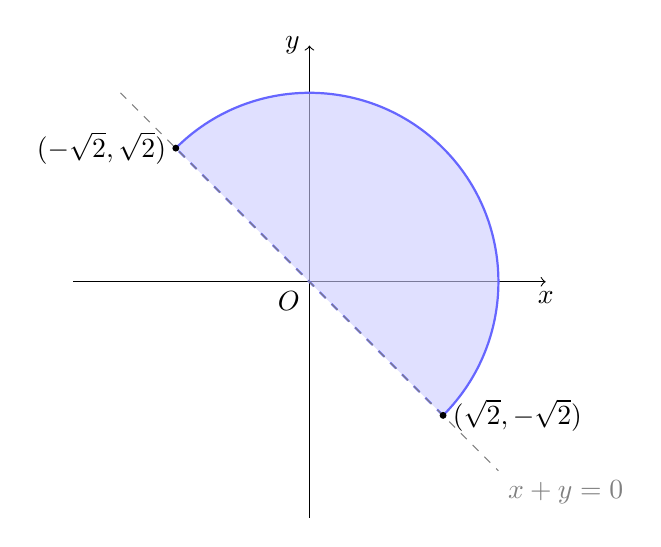
\begin{tikzpicture}[scale=1.2]
  
  % 坐标轴
  \draw[->] (-2.5,0) -- (2.5,0) node[below] {$x$};
  \draw[->] (0,-2.5) -- (0,2.5) node[left] {$y$};
  \node[below left] at (0,0) {$O$};

  % 填充区域：只填充不描边
  \path[fill=blue!20, opacity=0.6]
       (-45:2) arc[start angle=-45, end angle=135, radius=2]
       -- cycle;

  % 绘制圆弧边界（实线，表示包含边界）
  \draw[blue!60, thick]
       (-45:2) arc[start angle=-45, end angle=135, radius=2];

  % 绘制直线边界（虚线，表示 x+y>0 不包含边界）
  \draw[blue!60, thick, dashed]
       (-45:2) -- (135:2);

  % 整条直线 x+y=0（灰色虚线，作参照）
  \draw[gray, dashed, thin] (-2,2) -- (2,-2) node[below right] {$x+y=0$};

  % 标记两个交点
  \filldraw (135:2) circle[radius=0.03] node[left] {$(-\sqrt2,\sqrt2)$};
  \filldraw (-45:2) circle[radius=0.03] node[right] {$(\sqrt2,-\sqrt2)$};

\end{tikzpicture}
\end{center}

二元函数和一元函数的一个重要区别在于，一元函数的定义域是数轴上的区间，只有左右两个方向。二元函数的定义域是平面上的区域，可以从无穷多个方向趋近于同一点。正是这个区别，使得多元函数的极限比一元情形复杂得多。


\subsection{多元函数的极限}

在一元函数中，极限 $\lim_{x \to x_0} f(x) = L$ 的意思是，无论 $x$ 从左边还是右边趋近于 $x_0$，$f(x)$ 都趋近于 $L$。只有两条路可走，要么左要么右。

到了二元函数，情况就变了。$(x,y)$ 趋近于 $(x_0, y_0)$ 时，可以有无数条路径。因为平面上有无数条曲线可以从不同方向趋近于同一点。为了保证极限存在，必须保证沿着所有路径趋近时，函数值都趋近于同一个数。

\begin{definition}{二元函数的极限}{}
设函数 $z = f(x, y)$ 在 $(x_0, y_0)$ 的某个去心邻域内有定义，$L$ 为实数。若对于任意给定的 $\epsilon > 0$，总存在 $\delta > 0$，使得当
\[
0 < \sqrt{(x - x_0)^2 + (y - y_0)^2} < \delta
\]
时，就有
\[
|f(x, y) - L| < \epsilon
\]
则称当 $(x, y)$ 趋近于 $(x_0, y_0)$ 时，$f(x, y)$ 的\textbf{极限}为 $L$，记作
\[
\lim_{(x,y) \to (x_0, y_0)} f(x, y) = L
\]
\end{definition}

有没有发现这个定义和第二章的 $\epsilon-\delta$ 定义几乎一模一样？唯一的区别是 $|x - x_0|$ 被换成了两点间的距离 $\sqrt{(x - x_0)^2 + (y - y_0)^2}$。所以核心思想完全一致：\textbf{无论我把误差 $\epsilon$ 定得多小，你都能找到一个以 $(x_0, y_0)$ 为中心，半径为 $\delta$的小圆盘，只要 $(x, y)$ 进入这个圆盘，$f(x, y)$ 就一定落在 $L$ 的 $\epsilon$ 邻域内}。

但这个定义在实际计算中有一层隐藏的严格性，它要求极限值与趋近路径无关。也就是说，无论你沿着哪条曲线趋近于 $(x_0, y_0)$，得到的结果必须一样。

这就给了我们一个判断极限不存在的工具，\textbf{找两条不同的路径，如果极限值不同，就说明极限不存在}。

\begin{myexample}
  讨论 $f(x, y) = \dfrac{xy}{x^2 + y^2}$ 在 $(0, 0)$ 处的极限。

  沿着 $y = kx$趋近于原点，那么代入$y = kx$，我们有：
  \[
  f(x, kx) = \frac{x \cdot kx}{x^2 + (kx)^2} = \frac{kx^2}{x^2(1 + k^2)} = \frac{k}{1 + k^2}
  \]

  当 $(x, y) \to (0, 0)$ 时，这个值等于 $\frac{k}{1+k^2}$，它依赖 $k$ 的取值。因此极限不存在。
\end{myexample}

怎么理解呢？我们沿着 $y = x$得到极限值为 $\frac{1}{2}$，沿着 $y = 0$得到极限值为$0$。不同路径得到不同结果，就像一元函数里左极限不等于右极限一样，所以极限不存在。

再看一个例子：

\begin{myexample}
  讨论 $f(x, y) = \dfrac{x^2 y}{x^4 + y^2}$ 在 $(0, 0)$ 处的极限。

  沿着 $y = kx$ 趋近原点，那么代入$y = kx$，得：
  \[
  f(x, kx) = \frac{x^2 \cdot kx}{x^4 + (kx)^2} = \frac{kx^3}{x^4 + k^2 x^2} = \frac{kx}{x^2 + k^2}
  \]

  \[\lim_{x \to 0} \frac{kx}{x^2 + k^2} = \frac{0}{k^2} = 0\]

  沿着任意一条直线，极限都是 $0$。但这能说明极限就是 $0$ 吗？让我们试试抛物线 $y = x^2$，那么代入$y = x^2$，得：
  \[
  f(x, x^2) = \frac{x^2 \cdot x^2}{x^4 + (x^2)^2} = \frac{x^4}{x^4 + x^4} = \frac{1}{2}
  \]

  沿着抛物线取到的极限是 $\frac{1}{2}$，而直线是 $0$。所以极限还是不存在。
\end{myexample}

这个例子说明，沿着所有直线极限都相同，不意味着极限存在，因为还有曲线路径。所以在二元函数中，要证明极限存在，必须用定义严格证明。要证明极限不存在，找到两条不同路径得到不同结果即可。

和一元函数一样，二元函数的极限也有类似的运算律。若两个函数的极限都存在，则函数四则运算的极限等于极限的四则运算结果。证明方法也和一元完全类似，此处不再重复。

\subsection{多元函数的连续性}

和一元情形一样，连续性的定义就是把极限中的 $L$ 换成函数值 $f(x_0, y_0)$，并去掉“去心”条件。

\begin{definition}{二元函数的连续性}{}
设函数 $z = f(x, y)$ 在 $(x_0, y_0)$ 的某个邻域内有定义。若
\[
\lim_{(x,y) \to (x_0, y_0)} f(x, y) = f(x_0, y_0)
\]
则称 $f(x, y)$ 在点 $(x_0, y_0)$ 处\textbf{连续}。如果函数在区域 $D$ 上的每一点都连续，就称 $f(x, y)$ 在 $D$ 上连续。
\end{definition}

这个定义拆开来看就是三个条件，$f(x_0, y_0)$ 有定义，极限 $\lim_{(x,y) \to (x_0, y_0)} f(x, y)$ 存在，极限等于函数值。三者缺一不可。这也和一元函数极限与连续的关系完全一样。因此之前在一元函数成立的定理在二元函数仍然适用，包括：

\begin{theorem}{多元初等函数的连续性}{}
  多元初等函数在其定义域内都是连续的。
\end{theorem}

这里的多元初等函数和一元初等函数类似，由一个解析表达式定义，包含多项式、有理函数、根式、指数对数、三角函数、反三角函数等，以及它们经有限次四则运算和复合得出的函数。

\begin{theorem}{连续函数的运算性质}{}
若 $f(x, y)$ 和 $g(x, y)$ 都在 $(x_0, y_0)$ 处连续，则
\[
f \pm g,\quad f \cdot g,\quad \frac{f}{g}\ (g \neq 0)
\]
都在 $(x_0, y_0)$ 处连续。
\end{theorem}


\begin{theorem}{有界性定理}{}
若 $f(x, y)$ 在有界闭区域 $D$ 上连续，则$f(x, y)$ 在 $D$ 上有界。
\end{theorem}

\begin{theorem}{最值定理}{}
  若 $f(x, y)$ 在有界闭区域 $D$ 上连续，则$f(x, y)$ 在 $D$ 上能取到最大值和最小值。
\end{theorem}

\begin{theorem}{介值定理}{}
若 $f(x, y)$ 在区域 $D$ 上连续，$P_1, P_2 \in D$ 且 $f(P_1) < f(P_2)$，则对于 $f(P_1)$ 与 $f(P_2)$ 之间的任意一个数 $\mu$，都存在至少一个点 $P_\xi \in D$，使得 $f(P_\xi) = \mu$。
\end{theorem}

这些性质和一元闭区间上的连续性性质如出一辙，核心条件都是“有界闭区域”加“连续”。反过来，如果区域不是闭的或者函数不连续，这些结论就不保证成立。这些定理本质上和一元函数完全一致，只是从一维推广到二维。从闭区间推广到有界闭区域。

\section{偏导数}
在一元函数中，导数 $f'(x)$ 描述了函数值随自变量变化的快慢。对于二元函数 $z = f(x,y)$，我们自然也想考察函数值随自变量变化的情况。但是自变量有两个，怎么处理呢？

\subsection{偏导数及其几何意义}
面对两个自变量，核心思想是先固定一个，再看另一个。因为二元函数 $z = f(x,y)$的自变量在平面上可以沿无数个方向变化，但我们没法一次性把所有这些方向都研究完。所以，我们只能分别看沿坐标轴方向的变化。于是，我们就引出了偏导数：

\begin{definition}{偏导数}{}
设函数 $z = f(x,y)$ 在点 $(x_0, y_0)$ 的某邻域内有定义。

若极限
\[
\lim_{\Delta x \to 0} \frac{f(x_0 + \Delta x, y_0) - f(x_0, y_0)}{\Delta x}
\]
存在，则称此极限为 $f(x,y)$ 在点 $(x_0, y_0)$ 处\textbf{对 $x$ 的偏导数}，记作
\[
\frac{\partial z}{\partial x}\Big|_{(x_0,y_0)},\quad \frac{\partial f}{\partial x}\Big|_{(x_0,y_0)},\quad f_x(x_0,y_0),\quad \text{或}\quad z_x(x_0,y_0)
\]

若极限
\[
\lim_{\Delta y \to 0} \frac{f(x_0, y_0 + \Delta y) - f(x_0, y_0)}{\Delta y}
\]
存在，则称此极限为 $f(x,y)$ 在点 $(x_0, y_0)$ 处\textbf{对 $y$ 的偏导数}，记作
\[
\frac{\partial z}{\partial y}\Big|_{(x_0,y_0)},\quad \frac{\partial f}{\partial y}\Big|_{(x_0,y_0)},\quad f_y(x_0,y_0),\quad \text{或}\quad z_y(x_0,y_0)
\]
\end{definition}

这个定义和一元导数的定义长得几乎一模一样，唯一的区别是求对 $x$ 的偏导数时，把 $y$ 固定为 $y_0$，只让 $x$ 变化。求对 $y$ 的偏导数时，把 $x$ 固定为 $x_0$，只让 $y$ 变化。换句话说，\textbf{偏导数就是把其他变量视作常数后，对该变量求一元导数}。

因此，偏导数的计算法则其实非常直接。对哪个变量求导，就把其余变量当作常数，然后利用一元函数的所有求导公式和法则。

来看一个例子：

\begin{myexample}
设 $z = x^3y + 2x^2 + e^{xy}$，求 $\frac{\partial z}{\partial x}$ 和 $\frac{\partial z}{\partial y}$。

对 $x$ 求偏导时，把 $y$ 当作常数：
\[
\frac{\partial z}{\partial x} = 3x^2 \cdot y + 4x + e^{xy} \cdot y = 3x^2y + 4x + y e^{xy}
\]

对 $y$ 求偏导时，把 $x$ 当作常数：
\[
\frac{\partial z}{\partial y} = x^3 \cdot 1 + 0 + e^{xy} \cdot x = x^3 + x e^{xy}
\]
\end{myexample}

是不是很简单？所谓偏导数，本质上就是“假装”其他变量是常数，然后用一元导数的方法去算。

接下来看几何意义。在一元函数中，导数 $f'(x_0)$ 是曲线 $y = f(x)$ 在点 $(x_0, f(x_0))$ 处切线的斜率。二元函数 $z = f(x,y)$ 的图像是空间中的一张曲面，偏导数 $f_x(x_0,y_0)$ 和 $f_y(x_0,y_0)$ 也对应着切线的斜率，只不过需要用平面去截曲面，再退化成二维曲线来看。

固定 $y = y_0$，平面 $y = y_0$ 与曲面 $z = f(x,y)$ 相交，得到一条曲线
\[
C_x:\; z = f(x, y_0), \quad y = y_0
\]

这条曲线可以看作关于 $x$ 的一元函数。它在点 $P_0(x_0, y_0, f(x_0, y_0))$ 处的切线对 $x$ 轴的斜率，正好就是偏导数 $f_x(x_0, y_0)$。同样，固定 $x = x_0$，平面 $x = x_0$ 与曲面相交得到曲线
\[
C_y:\; z = f(x_0, y), \quad x = x_0
\]

该曲线在 $P_0$ 处的切线对 $y$ 轴的斜率就是偏导数 $f_y(x_0, y_0)$。

简而言之，\textbf{偏导数 $f_x$ 衡量的是曲面沿 $x$ 轴方向的变化趋势，$f_y$ 衡量的是曲面沿 $y$ 轴方向的变化趋势。} 曲面被坐标面“切开”后，我们看到的正是两个一元函数，因此偏导数的几何意义与一元导数其实是一脉相承的。

\begin{center}
  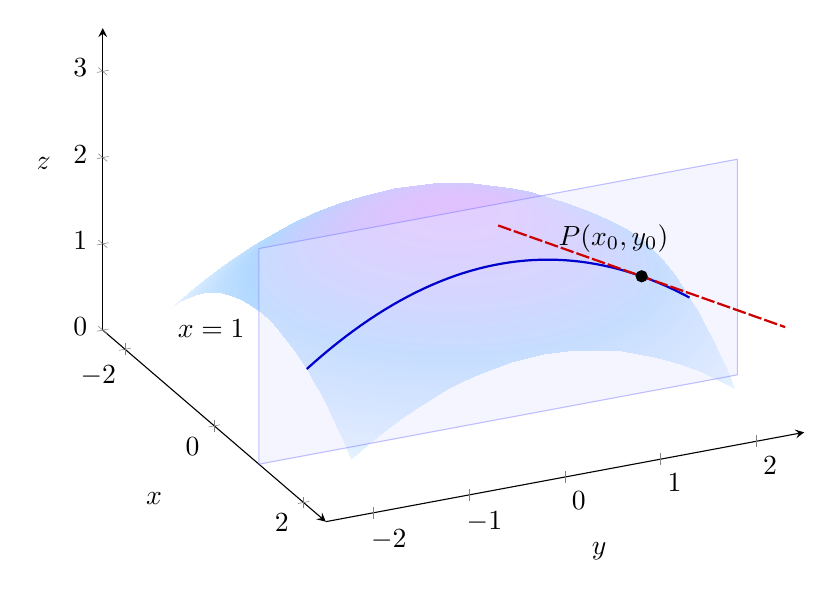
\begin{tikzpicture}
  \begin{axis}[
      scale=1.3,
      view={65}{35},
      xmin=-2.5, xmax=2.5,
      ymin=-2.5, ymax=2.5,
      zmin=0, zmax=3.5,
      xlabel=$x$, ylabel=$y$, zlabel=$z$,
      zlabel style={rotate=90},
      axis lines=left,
      colormap/cool,
      clip=false
  ]
  
  % 绘制曲面 z = f(x,y) = 2 - 0.2(x^2 + y^2)
  \addplot3[
      surf,
      shader=interp, 
      domain=-2:2, 
      y domain=-2:2, 
      opacity=0.3, 
      faceted color=black!30
  ] {2 - 0.2*(x^2 + y^2)};
  
  % 用 x = 1 的平面“切开”曲面（对应 y 方向的偏导）
  \addplot3[
      surf, 
      mesh/rows=2, 
      shader=flat, 
      draw=blue!60, 
      fill=blue!10, 
      opacity=0.4
  ] coordinates {(1,-2.5,0) (1,2.5,0) (1,-2.5,2.5) (1,2.5,2.5)};
  
  % 绘制“切痕”曲线 C_y (平面 x=1 与曲面的交线)
  \addplot3[
      domain=-2:2, 
      samples=50, 
      thick, 
      blue!80!black
  ] ({1}, {y}, {2 - 0.2*(1^2 + y^2)});
  
  % 绘制切线 T_y (斜率 = f_y)
  \addplot3[
      domain=-1.5:1.5, 
      samples=2, 
      dashed, 
      thick, 
      red!80!black
  ] ({1}, {1.5+x}, {1.35 - 0.6*x});
  
  % 标记切点 P(x0, y0)
  \addplot3[only marks, mark=*, mark size=2, black] coordinates {(1,1.5,1.35)};
  
  \node[label={[label distance=0.2cm]135:{$P(x_0,y_0)$}}] at (1,2.1,1.15) {};
  
  \node[label={$x=1$}] at (1,-3,1.35) {};
  
  \end{axis}
  \end{tikzpicture}
\end{center}

上图的例子就很好展现了偏导数的几何意义。曲面被平面 $x = 1$ 截出一条蓝色曲线，在点 $P(x_0,y_0)$ 处，该曲线沿 $y$ 轴的红色切线斜率就是 $\frac{\partial z}{\partial y}$。

有了偏导数的几何直观，我们就可以研究二元函数沿坐标轴方向的变化率了。不过要注意，这只是两个特殊方向，沿着$x$和沿着$y$的方向，并不能代表所有方向的变化率。偏导数只反映沿坐标轴方向的信息，无法控制其他路径的行为。这暗示了多元函数的偏导存在和连续性之间的关系比一元函数复杂得多。

回想我们之前讨论过的函数：

\begin{myexample}
  函数\(f(x,y) = \frac{xy}{x^2 + y^2}\)补充定义 $f(0,0)=0$，讨论$f(x,y)$的连续性。

补充定义 $f(0,0)=0$后函数表述为：
\[
f(x,y) = \begin{cases}
\frac{xy}{x^2 + y^2}, & (x,y) \neq (0,0) \\
0, & (x,y) = (0,0)
\end{cases}
\]

根据偏导数定义：
\[
f_x(0,0) = \lim_{\Delta x\to0}\frac{f(\Delta x,0)-f(0,0)}{\Delta x} = 0
\]
\[
f_y(0,0) = \lim_{\Delta y\to0}\frac{f(0,\Delta y)-f(0,0)}{\Delta y} = 0
\]

两个偏导数都存在且为 $0$。但我们已经证明过，$(x,y)\to(0,0)$ 时该函数的极限根本不存在，自然也就不连续。
\end{myexample}

这个反例说明，在多元函数中，\textbf{偏导数存在并不能保证函数连续}。这一点和一元函数截然不同，需要特别记忆。

\subsection{高阶偏导数}

偏导数 $f_x(x,y)$ 和 $f_y(x,y)$ 本身仍然是 $x,y$ 的二元函数。如果它们对 $x$ 或 $y$ 再次可求偏导，我们就得到\textbf{二阶偏导数}。依此类推，还可以定义三阶、四阶乃至更高阶的偏导数。

\begin{definition}{高阶偏导数的记号}{}
设函数 $z = f(x, y)$ 具有任意阶偏导数，其高阶偏导数用以下记号表示：

拉格朗日记号：
\[
f_x,\ f_y,\quad 
f_{xx},\ f_{xy},\ f_{yx},\ f_{yy},\quad 
f_{xxx},\ f_{xxy},\ f_{xyx},\ \dots,\ 
f_{\underbrace{x\cdots x}_{p}\,\underbrace{y\cdots y}_{q}}
\]

莱布尼茨记号：
\[
\frac{\partial z}{\partial x},\ \frac{\partial z}{\partial y},\quad 
\frac{\partial^2 z}{\partial x^2},\ \frac{\partial^2 z}{\partial x\partial y},\ \frac{\partial^2 z}{\partial y\partial x},\ \frac{\partial^2 z}{\partial y^2},\quad \frac{\partial^3 z}{\partial x^3},\ \frac{\partial^3 z}{\partial x^2\partial y},\ \frac{\partial^3 z}{\partial x\partial y\partial x},\ \dots,\ \frac{\partial^{p+q} z}{\partial x^p\,\partial y^q}
\]
其中 $f_{xy}$ 、 $f_{yx}$ 、 $f_{xyx}$ 等称为\textbf{混合偏导数}。
\end{definition}

混合偏导数有求导次序的区别，$f_{xy}$ 表示先对 $x$ 再对 $y$ 求偏导，$f_{yx}$ 表示先对 $y$ 再对 $x$ 求偏导。也就是谁放前面就对谁先求偏导。

有时我们也用$f_1$，$f_2$ 等来表示一阶偏导数，用 $f_{11}$，$f_{12}$ 等来表示二阶偏导数。$f_1$表示对第一个变量求偏导，$f_{12}$表示先对第一个变量求偏导再对第二个变量求偏导。$f_{11}$，$f_{12}$以此类推。这种记法在抽象函数里很常见。

计算高阶偏导数并没有新技巧，就是老老实实一次又一次地用一元求导法则，记住每次只对一个变量求导，其他变量视为常数。看一个例子：

\begin{myexample}
设 $z = x^3y^2 + \sin xy$，求所有二阶偏导数。

先算一阶偏导：
\[
\frac{\partial z}{\partial x} = 3x^2y^2 + y\cos xy,\qquad
\frac{\partial z}{\partial y} = 2x^3y + x\cos xy
\]

再对每个一阶偏导继续求偏导：
\begin{align*}
\frac{\partial^2 z}{\partial x^2}
&= \frac{\partial}{\partial x}(3x^2y^2 + y\cos xy)
= 6xy^2 - y^2\sin xy \\[4pt]
\frac{\partial^2 z}{\partial x\partial y}
&= \frac{\partial}{\partial y}(3x^2y^2 + y\cos xy)
= 6x^2y + \cos xy - xy\sin xy \\[4pt]
\frac{\partial^2 z}{\partial y\partial x}
&= \frac{\partial}{\partial x}(2x^3y + x\cos xy)
= 6x^2y + \cos xy - xy\sin xy \\[4pt]
\frac{\partial^2 z}{\partial y^2}
&= \frac{\partial}{\partial y}(2x^3y + x\cos xy)
= 2x^3 - x^2\sin xy
\end{align*}
\end{myexample}

仔细观察结果，我们发现 $f_{xy}$ 和 $f_{yx}$ 结果一样。这说明，在某种条件下，混合偏导数的值与求导次序无关：

\begin{theorem}{克莱罗定理}{}
若函数 $z = f(x,y)$ 的两个混合偏导数 $f_{xy}$ 和 $f_{yx}$ 在区域 $D$ 内连续，则它们在 $D$ 内处处相等：
\[
f_{xy}(x,y) = f_{yx}(x,y)
\]
\end{theorem}

这个定理的意义在于，当我们看到对称出现的混合偏导时，只要它们连续，就可以放心地交换求导次序，不必担心结果不同。上面的例题正是由于 $\sin xy$ 无穷次可微，混合偏导数连续，自然满足这个定理。

对于更高阶的偏导数，比如 $f_{xxy}$，只要涉及的混合偏导数都连续，求导次序就可以任意排列。比如 $f_{xxy}$、$f_{xyx}$、$f_{yxx}$ 在连续条件下都相等。这使得我们在计算时可以灵活选择最方便的次序，往往能大幅简化运算。

高阶偏导数的几何意义不如一阶那样直观。一阶偏导数衡量曲面沿坐标轴的倾斜程度，二阶偏导数 $f_{xx}$ 和 $f_{yy}$ 则衡量这种倾斜本身变化的快慢，即曲面的\textbf{弯曲程度}。混合偏导数 $f_{xy}$ 反映了曲面在 $x$ 方向变化时，$y$ 方向的斜率如何变化，这可以理解为一种“扭转”。



\subsection{多元复合函数求偏导数}

在一元函数中，我们有链式法则。到了多元函数，复合的方式更加多样，自变量和中间变量都可以有多个，链式法则依然存在，只是要把所有“影响路径”都考虑进来。

我们从一个最典型的情形入手。设 $z = f(u,v)$ 是 $u,v$ 的函数，而 $u = u(x,y)$，$v = v(x,y)$ 又都是 $x,y$ 的函数。把它们复合起来，就得到 $z$ 关于 $x,y$ 的二元函数：
\[
z = f(u(x,y),\, v(x,y))
\]

现在要怎么求 $\frac{\partial z}{\partial x}$ 和 $\frac{\partial z}{\partial y}$呢？

直观上，$x$ 发生微小变化时，会同时引起 $u$ 和 $v$ 的变化，而这两个变化又会“传递”到 $z$。因此 $z$ 对 $x$ 的变化率应该是两条路径上变化率的叠加。把这种关系画出来，会得到一张“变量依赖关系图”：

\begin{center}
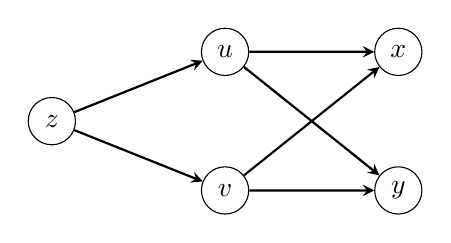
\begin{tikzpicture}[scale=1.1,
    >=stealth,
    var/.style={draw, circle, minimum size=6mm, inner sep=1pt},
    edge/.style={->, thick}]

  \node[var] (z) at (0, 0)    {$z$};
  \node[var] (u) at (2, 0.8)  {$u$};
  \node[var] (v) at (2,-0.8)  {$v$};
  \node[var] (x) at (4, 0.8)  {$x$};
  \node[var] (y) at (4,-0.8)  {$y$};

  \draw[edge] (z) -- (u);
  \draw[edge] (z) -- (v);
  \draw[edge] (u) -- (x);
  \draw[edge] (u) -- (y);
  \draw[edge] (v) -- (x);
  \draw[edge] (v) -- (y);
\end{tikzpicture}
\end{center}

也就是说，函数$z$ 依赖于中间变量$u$ 和 $v$，而$u$ 和 $v$又分别依赖于自变量 $x$和$y$。所以每一条从 $z$ 到 $x$ 的路径都对应着一种影响，例如$z \to u \to x$ 的影响是 $\frac{\partial z}{\partial u}\frac{\partial u}{\partial x}$，$z \to v \to x$ 的影响是 $\frac{\partial z}{\partial v}\frac{\partial v}{\partial x}$。所有这些影响加起来，就是 $z$ 对 $x$ 的总变化率。这个规律总结起来，就是多元复合函数求导的链式法则：

\begin{theorem}{多元函数链式法则}{}
设 $z = f(u,v)$ 在对应点 $(u,v)$ 处具有连续偏导数，$u = u(x,y)$，$v = v(x,y)$ 在点 $(x,y)$ 处具有连续偏导数，则复合函数 $z = f(u(x,y), v(x,y))$ 在 $(x,y)$ 处的偏导数存在，且：
\[
\frac{\partial z}{\partial x} = \frac{\partial z}{\partial u}\frac{\partial u}{\partial x} + \frac{\partial z}{\partial v}\frac{\partial v}{\partial x}
\]
\[
\frac{\partial z}{\partial y} = \frac{\partial z}{\partial u}\frac{\partial u}{\partial y} + \frac{\partial z}{\partial v}\frac{\partial v}{\partial y}
\]
\end{theorem}

这个公式说的是，\textbf{因变量对某个自变量的偏导数，等于所有从因变量通往该自变量的路径上偏导数乘积的总和。} 有多少条路径，就有多少项相加，每条路径经过几层，就乘上几个偏导数。

有了它，我们就能处理各种复杂的复合情形。

下面看几个例子：

\begin{myexample}
  设函数$z=u^2+v^2$，其中 $u = \sin t$，$v = \cos t$，求 $\frac{dz}{dt}$。

  先画出路径关系图：

\begin{center}
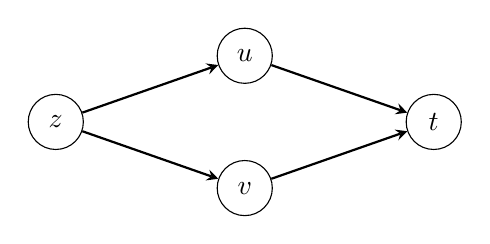
\begin{tikzpicture}[scale=1.2,
    >=stealth,
    var/.style={draw, circle, minimum size=7mm, inner sep=0pt},
    edge/.style={->, thick}]

  \node[var] (z) at (0,0)   {$z$};
  \node[var] (u) at (2,0.7) {$u$};
  \node[var] (v) at (2,-0.7){$v$};
  \node[var] (t) at (4,0)   {$t$};

  \draw[edge] (z) -- (u);
  \draw[edge] (z) -- (v);
  \draw[edge] (u) -- (t);
  \draw[edge] (v) -- (t);
\end{tikzpicture}
\end{center}

我们可以清晰地看到，$z$ 对 $t$ 的变化率有两条路径：$z \to u \to t$ 和 $z \to v \to t$。因此：
\[
\frac{dz}{dt} = \frac{\partial z}{\partial u}\frac{du}{dt} + \frac{\partial z}{\partial v}\frac{dv}{dt}
\]

所以：
\[
\frac{dz}{dt} = \frac{\partial z}{\partial u}\cos t - \frac{\partial z}{\partial v}\sin t
=2u\cos t-2v\sin t=2\sin t \cos t-2\cos t \sin t=0
\]
\end{myexample}

由这个例子我们得到，若 $z = f(u,v)$，而 $u = u(t)$，$v = v(t)$ 都只是一元函数，那么复合后 $z$ 就是 $t$ 的一元函数。此时对 $t$ 求导就是“全导数”：
\[
\frac{dz}{dt} = \frac{\partial z}{\partial u}\frac{du}{dt} + \frac{\partial z}{\partial v}\frac{dv}{dt}
\]

这是一元函数链式法则在多元中的直接推广。

不过，不是所有复合函数都要这样算，我们可以把 $u = \sin t$和$v = \cos t$代入到$z=u^2+v^2$里，化简后我们会发现$z=1$，因此导数自然是$0$了。


\begin{myexample}
  设函数$z=u^2+v^2$，其中 $u = x-y$，$v = x+y$，求 $\frac{\partial z}{\partial x}$ 和 $\frac{\partial z}{\partial y}$。

分析函数，$u$和$v$都是$x$和$y$的函数，所以$z$是$x$和$y$的函数。画出路径关系图：

\begin{center}
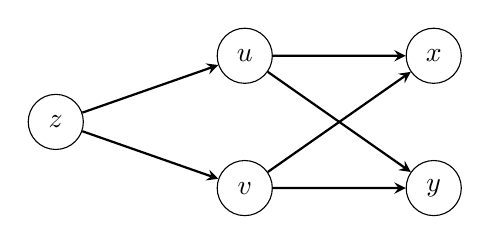
\begin{tikzpicture}[scale=1.2,
    >=stealth,
    var/.style={draw, circle, minimum size=7mm, inner sep=0pt},
    edge/.style={->, thick}]
    
  \node[var] (z) at (0,0)   {$z$};
  \node[var] (u) at (2,0.7) {$u$};
  \node[var] (v) at (2,-0.7){$v$};
  \node[var] (x) at (4,0.7) {$x$};
  \node[var] (y) at (4,-0.7){$y$};

  \draw[edge] (z) -- (u);
  \draw[edge] (z) -- (v);
  \draw[edge] (u) -- (x);
  \draw[edge] (u) -- (y);
  \draw[edge] (v) -- (x);
  \draw[edge] (v) -- (y);
\end{tikzpicture}
\end{center}

从图中可以看到，$z$ 对 $x$ 有两条路径：$z \to u \to x$ 和 $z \to v \to x$，对 $y$ 同样有两条路径：$z \to u \to y$ 和 $z \to v \to y$。因此：
  \[
  \frac{\partial z}{\partial x} = \frac{\partial z}{\partial u}\frac{\partial u}{\partial x}
    + \frac{\partial z}{\partial v}\frac{\partial v}{\partial x}
  \]
  \[
  \frac{\partial z}{\partial y} = \frac{\partial z}{\partial u}\frac{\partial u}{\partial y}
    + \frac{\partial z}{\partial v}\frac{\partial v}{\partial y}
  \]

  计算偏导数：
  \[
  \frac{\partial z}{\partial u} = 2u \quad \frac{\partial z}{\partial v} = 2v
  \quad
  \frac{\partial u}{\partial x} = 1 \quad \frac{\partial u}{\partial y} = -1
  \quad
  \frac{\partial v}{\partial x} = 1 \quad \frac{\partial v}{\partial y} = 1
  \]

  代入得：
  \begin{align*}
    \frac{\partial z}{\partial x}
    &= 2u \cdot 1 + 2v \cdot 1 = 2(u+v) \\
    &= 2[(x-y)+(x+y)] = 4x\\[4pt]
    \frac{\partial z}{\partial y}
    &= 2u \cdot (-1) + 2v \cdot 1 = 2(v-u) \\
    &= 2[(x+y)-(x-y)] = 4y
  \end{align*}

\end{myexample}

由这个例子我们发现，若 $z = f(u,v)$，而 $u = u(x,y)$，$v = v(x,y)$ 都是二元函数，那么复合后 $z$ 就是 $x,y$ 的二元函数。这时候就要用多元复合函数链式法则，画出路径关系图，找出所有从 $z$ 到自变量的路径，然后把每条路径上偏导数的乘积加起来。

\begin{myexample}
  设函数 $z = f(u+v, u-v)$，其中 $u = x$，$v = xy$，求 $\frac{\partial z}{\partial x}$ 和 $\frac{\partial z}{\partial y}$。

  分析函数，$z$ 通过 $u$ 和 $v$ 依赖于 $x,y$，其中 $u$ 仅依赖于 $x$，是$x$的一元函数，$v$ 依赖于 $x$ 和 $y$，是$x,y$的二元函数。画出路径关系图：
  \begin{center}
  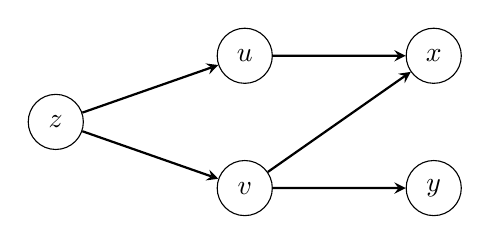
\begin{tikzpicture}[scale=1.2,
      >=stealth,
      var/.style={draw, circle, minimum size=7mm, inner sep=0pt},
      edge/.style={->, thick}]

    \node[var] (z) at (0,0)   {$z$};
    \node[var] (u) at (2,0.7) {$u$};
    \node[var] (v) at (2,-0.7){$v$};
    \node[var] (x) at (4,0.7) {$x$};
    \node[var] (y) at (4,-0.7){$y$};

    \draw[edge] (z) -- (u);
    \draw[edge] (z) -- (v);
    \draw[edge] (u) -- (x);
    \draw[edge] (v) -- (x);
    \draw[edge] (v) -- (y);
  \end{tikzpicture}
  \end{center}

  从图中可以看出，$z$ 对 $x$ 有两条路径：$z \to u \to x$ 和 $z \to v \to x$，对 $y$ 有一条路径：$z \to v \to y$，因此，由链式法则：
  \[
  \frac{\partial z}{\partial x} = \frac{\partial z}{\partial u}\frac{\partial u}{\partial x}
    + \frac{\partial z}{\partial v}\frac{\partial v}{\partial x}
  \]
  \[
  \frac{\partial z}{\partial y} = \frac{\partial z}{\partial v}\frac{\partial v}{\partial y}
  \]

  令 $p = u+v$, $q = u-v$，则 $z = f(p,q)$。由复合函数求导法则：
  \[
  \frac{\partial z}{\partial u} = \frac{\partial f}{\partial p}\frac{\partial p}{\partial u}
    + \frac{\partial f}{\partial q}\frac{\partial q}{\partial u}
    = f_1 \cdot 1 + f_2 \cdot 1 = f_1 + f_2
  \]
  \[
  \frac{\partial z}{\partial v} = \frac{\partial f}{\partial p}\frac{\partial p}{\partial v}
    + \frac{\partial f}{\partial q}\frac{\partial q}{\partial v}
    = f_1 \cdot 1 + f_2 \cdot (-1) = f_1 - f_2
  \]

  又由 $u = x$, $v = xy$ 得：
  \[
  \frac{\partial u}{\partial x} = 1,\quad \frac{\partial u}{\partial y} = 0,\quad
  \frac{\partial v}{\partial x} = y,\quad \frac{\partial v}{\partial y} = x
  \]

  代入链式法则公式：
  \begin{align*}
    \frac{\partial z}{\partial x}
    &= (f_1 + f_2) \cdot 1 + (f_1 - f_2) \cdot y \\
    &= f_1 + f_2 + y f_1 - y f_2 \\
    &= (1+y)f_1 + (1-y)f_2 \\[6pt]
    \frac{\partial z}{\partial y}
    &= (f_1 - f_2) \cdot x = x(f_1 - f_2)
  \end{align*}

  因为我们没有 $f$ 的显式，最终结果只能保留$f_1$和$f_2$，这也是常见的处理方式。
\end{myexample}

这个例子其实是三层复合抽象函数求偏导数，外层函数 $f$ 并没有给出具体表达式，只告诉我们 $z = f(u,v)$ 的某种结构。其中 \(f_1, f_2\) 分别是 \(f\) 对第一个中间变量 \(p\) 和第二个中间变量 \(q\) 的偏导数，它们仍是 \(u, v\) 的函数，即 \(f_1 = f_1(p,q),\; f_2 = f_2(p,q)\)。


\begin{myexample}
  设\(z = f(x^2 + y^2,\; e^{xy})\)，求 \(\frac{\partial^2 z}{\partial x^2}\) 和 \(\frac{\partial^2 z}{\partial y^2}\)。

  分析函数，令 \(u = x^2 + y^2\)，\(v = e^{xy}\)，则 \(z = f(u, v)\)。\(u\) 和 \(v\) 都是 \(x, y\) 的二元函数，\(z\) 通过 \(u, v\) 依赖于 \(x, y\)。画出路径关系图：

\begin{center}
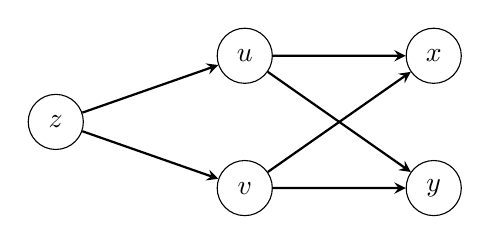
\begin{tikzpicture}[scale=1.2,
    >=stealth,
    var/.style={draw, circle, minimum size=7mm, inner sep=0pt},
    edge/.style={->, thick}]
    
  \node[var] (z) at (0,0)   {$z$};
  \node[var] (u) at (2,0.7) {$u$};
  \node[var] (v) at (2,-0.7){$v$};
  \node[var] (x) at (4,0.7) {$x$};
  \node[var] (y) at (4,-0.7){$y$};

  \draw[edge] (z) -- (u);
  \draw[edge] (z) -- (v);
  \draw[edge] (u) -- (x);
  \draw[edge] (u) -- (y);
  \draw[edge] (v) -- (x);
  \draw[edge] (v) -- (y);
\end{tikzpicture}
\end{center}

从图中可以看出，\(z\) 对 \(x\) 有两条路径 \(z \to u \to x\) 和 \(z \to v \to x\)，对 \(y\) 同样有两条路径 \(z \to u \to y\) 和 \(z \to v \to y\)。因此，由链式法则先求一阶偏导数：
\[
\frac{\partial z}{\partial x} = \frac{\partial f}{\partial u}\frac{\partial u}{\partial x} + \frac{\partial f}{\partial v}\frac{\partial v}{\partial x} = f_1 \cdot 2x + f_2 \cdot y e^{xy}
\]
\[
\frac{\partial z}{\partial y} = \frac{\partial f}{\partial u}\frac{\partial u}{\partial y} + \frac{\partial f}{\partial v}\frac{\partial v}{\partial y} = f_1 \cdot 2y + f_2 \cdot x e^{xy}
\]

计算二阶偏导数。先求 \(\dfrac{\partial^2 z}{\partial x^2}\)，对 \(\dfrac{\partial z}{\partial x}\) 再求关于 \(x\) 偏导：
\[
\frac{\partial^2 z}{\partial x^2} = \frac{\partial}{\partial x}(2x f_1 + y e^{xy} f_2)
\]

注意 \(f_1, f_2\) 对 \(x\) 求导时仍需用链式法则：
\[
\frac{\partial f_1}{\partial x} = \frac{\partial f_1}{\partial u}\frac{\partial u}{\partial x} + \frac{\partial f_1}{\partial v}\frac{\partial v}{\partial x} = f_{11}\cdot 2x + f_{12}\cdot y e^{xy}
\]
\[
\frac{\partial f_2}{\partial x} = \frac{\partial f_2}{\partial u}\frac{\partial u}{\partial x} + \frac{\partial f_2}{\partial v}\frac{\partial v}{\partial x} = f_{21}\cdot 2x + f_{22}\cdot y e^{xy}
\]

其中 \(f_{11}, f_{12}, f_{21}, f_{22}\) 为 \(f\) 的二阶偏导数。代入计算：
\begin{align*}
\frac{\partial^2 z}{\partial x^2}
&= 2f_1 + 2x\frac{\partial f_1}{\partial x} + \frac{\partial}{\partial x}(y e^{xy})\cdot f_2 + y e^{xy}\frac{\partial f_2}{\partial x} \\
&= 2f_1 + 2x(2x f_{11} + y e^{xy} f_{12}) + y^2 e^{xy} f_2 + y e^{xy}(2x f_{21} + y e^{xy} f_{22}) \\
&= 2f_1 + y^2 e^{xy} f_2 + 4x^2 f_{11} + 2xy e^{xy} f_{12} + 2xy e^{xy} f_{21} + y^2 e^{2xy} f_{22}
\end{align*}

由于混合偏导数连续，有 \(f_{12} = f_{21}\)，合并得：
\[
\frac{\partial^2 z}{\partial x^2} = 2f_1 + y^2 e^{xy} f_2 + 4x^2 f_{11} + 4xy e^{xy} f_{12} + y^2 e^{2xy} f_{22}
\]

再求 \(\dfrac{\partial^2 z}{\partial y^2}\)，对 \(\dfrac{\partial z}{\partial y}\) 求关于 \(y\) 偏导：
\[
\frac{\partial^2 z}{\partial y^2} = \frac{\partial}{\partial y}(2y f_1 + x e^{xy} f_2)
\]

\(f_1, f_2\) 对 \(y\) 的偏导数为：
\[
\frac{\partial f_1}{\partial y} = f_{11}\cdot 2y + f_{12}\cdot x e^{xy},\quad
\frac{\partial f_2}{\partial y} = f_{21}\cdot 2y + f_{22}\cdot x e^{xy}
\]

其中 \(\frac{\partial}{\partial y}(x e^{xy}) = x^2 e^{xy}\)。代入：
\begin{align*}
\frac{\partial^2 z}{\partial y^2}
&= 2f_1 + 2y\frac{\partial f_1}{\partial y} + x^2 e^{xy} f_2 + x e^{xy}\frac{\partial f_2}{\partial y} \\
&= 2f_1 + 2y(2y f_{11} + x e^{xy} f_{12}) + x^2 e^{xy} f_2 + x e^{xy}(2y f_{21} + x e^{xy} f_{22}) \\
&= 2f_1 + x^2 e^{xy} f_2 + 4y^2 f_{11} + 2xy e^{xy} f_{12} + 2xy e^{xy} f_{21} + x^2 e^{2xy} f_{22}
\end{align*}

利用 \(f_{12} = f_{21}\) 合并，得：
\[
\frac{\partial^2 z}{\partial y^2} = 2f_1 + x^2 e^{xy} f_2 + 4y^2 f_{11} + 4xy e^{xy} f_{12} + x^2 e^{2xy} f_{22}
\]

\end{myexample}

这个例子其实是复合函数求二阶偏导数，虽然很复杂，但是思路是清晰的，就是不断使用链式法则求导，找出所有从因变量到自变量的路径，然后把每条路径上偏导数的乘积加起来。

\begin{myexample}
  设函数 $z = f(u,v,w)$，其中 $u = x^2 + y^2$，$v = e^x$，$w = \ln y$，求 $\frac{\partial^2 z}{\partial x \partial y}$。

  分析函数，\(u\) 依赖于 \(x,y\)，\(v\) 仅依赖于 \(x\)，\(w\) 仅依赖于 \(y\)。画出路径关系图：

\begin{center}
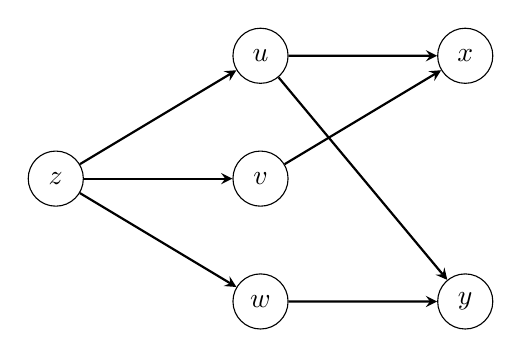
\begin{tikzpicture}[scale=1.3,
    >=stealth,
    var/.style={draw, circle, minimum size=7mm, inner sep=0pt},
    edge/.style={->, thick}]
    
  \node[var] (z) at (0,0)    {$z$};
  \node[var] (u) at (2,1.2)  {$u$};
  \node[var] (v) at (2,0)    {$v$};
  \node[var] (w) at (2,-1.2) {$w$};
  \node[var] (x) at (4,1.2)  {$x$};
  \node[var] (y) at (4,-1.2) {$y$};

  \draw[edge] (z) -- (u);
  \draw[edge] (z) -- (v);
  \draw[edge] (z) -- (w);
  \draw[edge] (u) -- (x);
  \draw[edge] (u) -- (y);
  \draw[edge] (v) -- (x);
  \draw[edge] (w) -- (y);
\end{tikzpicture}
\end{center}

从图中可以看出：\(z\) 对 \(x\) 有两条路径：\(z \to u \to x\)，\(z \to v \to x\)。\(z\) 对 \(y\) 有两条路径：\(z \to u \to y\)，\(z \to w \to y\)。

由链式法则，先计算一阶偏导：
\[
\frac{\partial z}{\partial x} = \frac{\partial z}{\partial u} \frac{\partial u}{\partial x} + \frac{\partial z}{\partial v} \frac{d v}{d x}
= f_1 \cdot 2x + f_2 \cdot e^x = 2x f_1 + e^x f_2
\]
\[
\frac{\partial z}{\partial y} = \frac{\partial z}{\partial u} \frac{\partial u}{\partial y} + \frac{\partial z}{\partial w} \frac{d w}{d y}
= f_1 \cdot 2y + f_3 \cdot \frac{1}{y} = 2y f_1 + \frac{1}{y} f_3
\]

下面求混合偏导数 \(\dfrac{\partial^2 z}{\partial x \partial y} = \dfrac{\partial}{\partial y}\!\left(\dfrac{\partial z}{\partial x}\right)\)。对 \(2x f_1 + e^x f_2\) 关于 \(y\) 求偏导时，\(2x\) 与 \(e^x\) 与 \(y\) 无关，视为系数：
\[
\frac{\partial^2 z}{\partial x \partial y} = 2x \frac{\partial f_1}{\partial y} + e^x \frac{\partial f_2}{\partial y}
\]

现在求 \(f_1\) 和 \(f_2\) 对 \(y\) 的偏导数。它们通过中间变量 \(u,v,w\) 依赖于 \(y\)，但 \(v\) 与 \(y\) 无关，因此链式法则中只出现 \(u\) 和 \(w\) 的路径：
\[
\frac{\partial f_1}{\partial y} = \frac{\partial f_1}{\partial u}\frac{\partial u}{\partial y} + \frac{\partial f_1}{\partial w}\frac{\partial w}{\partial y},
\qquad
\frac{\partial f_2}{\partial y} = \frac{\partial f_2}{\partial u}\frac{\partial u}{\partial y} + \frac{\partial f_2}{\partial w}\frac{\partial w}{\partial y}
\]

代入 \(\frac{\partial u}{\partial y} = 2y\)，\(\frac{\partial w}{\partial y} = \frac{1}{y}\)，得：
\[
\frac{\partial f_1}{\partial y} = f_{11} \cdot 2y + f_{13} \cdot \frac{1}{y},\qquad
\frac{\partial f_2}{\partial y} = f_{21} \cdot 2y + f_{23} \cdot \frac{1}{y}
\]

将上述结果代回，整理得：
\begin{align*}
\frac{\partial^2 z}{\partial x \partial y}
&= 2x( 2y f_{11} + \frac{1}{y} f_{13} ) + e^x( 2y f_{21} + \frac{1}{y} f_{23} ) \\
&= 4xy f_{11} + \frac{2x}{y} f_{13} + 2y e^x f_{21} + \frac{e^x}{y} f_{23}
\end{align*}

因为没有 \(f\) 的显式，最终结果保留二阶偏导记号，它们仍然都是 \(u = x^2 + y^2\)，\(v = e^x\)，\(w = \ln y\) 的函数。
\end{myexample}

这是一个三元的函数，但是只要我们抓住路径关系图，找出所有从因变量到自变量的路径，即使是无限元函数我们也能求偏导数。

最后要说明的是，对 $u$ 求偏导，把$v$看作常数，与 $u$ 最终依赖什么自变量毫无关系。最终代入 $u,v$ 关于 $x,y$ 的表达式时，才真正显含 $x,y$。每次求偏导时，都把其他变量视为常数，就不会出错。

多元复合函数求偏导数的链式法则，是整个多元微分学运算的骨架。它来源于一元函数，但比一元函数复杂。只要掌握了它，就能处理各种复杂的复合函数求偏导数问题。

\subsection{隐函数求偏导数}

有时变量之间的关系常常不是以 $y = f(x)$ 或 $z = f(x,y)$ 这种显式给出的，而是以隐函数的形式给出。例如我们之前学过的一元隐函数$F(x, y) = 0$，虽然不能简单地解出 $y$ 关于 $x$ 的初等函数表达式，但在一定条件下，它仍然确定了一个 $y$ 对 $x$ 的函数。我们现在要研究如何直接从方程本身求出这个“隐藏”函数的偏导数。

我们先从我们学过的一元隐函数入手。设方程$F(x, y) = 0$在某个区域内确定了一个函数 $y = y(x)$。也就是说，把 $y(x)$ 代入后，$F(x, y(x)) = 0$ 是一个恒等式。我们的目标是求 $\dfrac{dy}{dx}$，而不必先解出 $y$ 的显式。

现在我们有了链式法则和偏导数，这个想法实施起来就很简单了。把 $F(x,y)$ 看作 $x$ 和 $y$ 的二元函数，而 $y$ 又是 $x$ 的函数。对恒等式 $F(x, y(x)) = 0$ 两边关于 $x$ 求偏导，根据链式法则，有：
\[
\frac{\partial F}{\partial x} \cdot 1 + \frac{\partial F}{\partial y} \cdot \frac{dy}{dx} = 0
\]

也就是：
\[
F_x + F_y \cdot y' = 0
\]

只要 $F_y \neq 0$，就可以解出：
\[
\frac{dy}{dx} = -\frac{F_x}{F_y}
\]

这就是一元隐函数的求导公式。

\begin{theorem}{一元隐函数求导公式}{}
  设方程 $F(x, y) = 0$ 在某个区间内确定了一个隐函数 $y = y(x)$，则
  \[
  \frac{dy}{dx} = -\frac{F_x}{F_y}
  \]
\end{theorem}

接下来看一个例子：

\begin{myexample}
设方程 $e^y + xy = 0$ 确定了函数 $y = y(x)$，求 $\dfrac{dy}{dx}$。

令 $F(x, y) = e^y + xy$，则：
\[
F_x = y,\qquad F_y = e^y + x
\]

代入公式，得：
\[
\frac{dy}{dx} = -\frac{F_x}{F_y} = -\frac{y}{e^y + x}
\]
\end{myexample}

这就是我们在第二章里说的，除了方程两边对$x$求导外，求隐函数导数的更强大的工具。

现在推广到二元隐函数，设方程$F(x, y, z) = 0$在某个区域内确定了一个函数 $z = z(x, y)$，即 $F(x, y, z(x,y)) = 0$。我们现在要求 $\dfrac{\partial z}{\partial x}$ 和 $\dfrac{\partial z}{\partial y}$，怎么做呢？

和一元隐函数的操作一样，我们把 $F(x,y,z)$ 看作三元函数，而 $z$ 是 $x$ 和 $y$ 的函数。固定 $y$，对恒等式两边关于 $x$ 求偏导，链式法则出手：
\[
\frac{\partial F}{\partial x} \cdot 1 + \frac{\partial F}{\partial y} \cdot 0 + \frac{\partial F}{\partial z} \cdot \frac{\partial z}{\partial x} = 0
\]

也就是：
\[
F_x + F_z \frac{\partial z}{\partial x} = 0
\]

类似地，固定 $x$ 对 $y$ 求偏导，得到：
\[
F_y + F_z \frac{\partial z}{\partial y} = 0
\]

因此，只要 $F_z \neq 0$，就有：
\[
\frac{\partial z}{\partial x} = -\frac{F_x}{F_z},\qquad
\frac{\partial z}{\partial y} = -\frac{F_y}{F_z}
\]

这就是二元隐函数的求偏导公式。

\begin{theorem}{二元隐函数求导公式}{}
  设方程 $F(x,y,z)$ 在某个区域内确定了一个隐函数 $z = z(x,y)$，则
\[
\frac{\partial z}{\partial x} = -\frac{F_x}{F_z},\qquad
\frac{\partial z}{\partial y} = -\frac{F_y}{F_z}
\]
\end{theorem}

直观上说，求 $\dfrac{\partial z}{\partial x}$ 时，把 $y$ 当成常数，然后按照一元隐函数的方式处理即可。

接下来看一个例子：

\begin{myexample}
设方程 $x^2 + y^2 + z^2 = 4$ 在 $z > 0$ 时确定了隐函数 $z = z(x,y)$，求 $\dfrac{\partial z}{\partial x}$ 和 $\dfrac{\partial z}{\partial y}$。

令 $F(x, y, z) = x^2 + y^2 + z^2 - 4$，则有：
\[
F_x = 2x,\quad F_y = 2y,\quad F_z = 2z
\]

因此：
\[
\frac{\partial z}{\partial x} = -\frac{2x}{2z} = -\frac{x}{z},\qquad
\frac{\partial z}{\partial y} = -\frac{2y}{2z} = -\frac{y}{z}
\]

这个结果和从显式 $z = \sqrt{4 - x^2 - y^2}$ 直接求偏导的结果完全一样。读者可自行验证。
\end{myexample}

这种方法的最大优点是，即使 $F(x,y,z)=0$ 无法解出 $z$ 的显式，也能求出偏导数。例如方程 $z + e^z = xy$，根本无法写出 $z$ 的初等表达式，但我们可以轻易求出偏导。

\begin{myexample}
设方程 $z + e^z = xy$ 确定了隐函数 $z = z(x,y)$，求 $\dfrac{\partial z}{\partial x}$ 和 $\dfrac{\partial z}{\partial y}$。

令 $F(x, y, z) = z + e^z - xy$，则有：
\[
F_x = -y,\quad F_y = -x,\quad F_z = 1 + e^z
\]

于是：
\[
\frac{\partial z}{\partial x} = -\frac{-y}{1 + e^z} = \frac{y}{1 + e^z},\qquad
\frac{\partial z}{\partial y} = -\frac{-x}{1 + e^z} = \frac{x}{1 + e^z}
\]
\end{myexample}

如果还需要求二阶偏导数，就在一阶偏导数的基础上再求一次偏导，此时要注意一阶偏导的表达式里可能仍含有 $z$，而 $z$ 本身又是 $x,y$ 的函数，需要再次使用链式法则。

\begin{myexample}
设方程 $z + e^z = xy$ 确定了隐函数 $z = z(x,y)$，求 $\dfrac{\partial^2 z}{\partial x^2}$。

已知 $\dfrac{\partial z}{\partial x} = \dfrac{y}{1 + e^z}$，再对 $x$ 求偏导：

\begin{align*}
\frac{\partial^2 z}{\partial x^2}
&= \frac{\partial}{\partial x}( \frac{y}{1 + e^z} )
 = y \cdot \frac{-\; e^z \frac{\partial z}{\partial x}}{(1 + e^z)^2} \\
&= -\frac{y e^z}{(1 + e^z)^2} \cdot \frac{y}{1 + e^z}
 = -\frac{y^2 e^z}{(1 + e^z)^3}
\end{align*}

这样我们就求得了二阶偏导数。
\end{myexample}

隐函数求偏导的方法与前面多元复合函数链式法则是一脉相承的。我们可以这样总结：

面对一个方程，认定哪些是自变量，哪些是因变量，然后对等式两边关于某个自变量求偏导，因变量求导时按照链式法则展开，最后解出所需的偏导数。


\section{全微分}
与偏导数对应的，我们有全微分。顾名思义，它是函数在一点处因所有自变量同时微小变化所引起的全部微分。偏导数，就是偏向某个变量的导数。全微分，就是全部变量的微分。

\subsection{函数可微的条件}

在一元函数中，可导和可微是等价的，导数存在也就意味着微分存在。但在多元函数中，情况要微妙得多。

让我们先回忆一下一元可微的定义：$f(x)$ 在 $x_0$ 处可微，是指存在常数 $A$ 使得当$\Delta x \to 0$时，
$\Delta y = A \cdot \Delta x + o(\Delta x)$，其中这个 $A$ 就是 $f'(x_0)$。推广到二元函数，我们自然希望：
\[
\Delta z = A \cdot \Delta x + B \cdot \Delta y + o\!(\sqrt{(\Delta x)^2 + (\Delta y)^2})
\]

其中 $A$ 和 $B$ 是两个偏导数 $f_x$ 和 $f_y$。那么我们仿照一元函数，可以定义：

\begin{definition}{全微分的定义}{}
设函数 $z = f(x, y)$ 在 $(x_0, y_0)$ 的某个邻域内有定义。记自变量的增量为 $\Delta x$和$\Delta y$，函数值的增量为$\Delta z$，自变量的增量$(\Delta x,\Delta y)$的模长为$\rho$，则：
  \[
  \Delta z = f(x_0+\Delta x, y_0+\Delta y)
  \]
  \[
  \rho = \sqrt{(\Delta x)^2 + (\Delta y)^2}
  \]
  如果存在两个与 $\Delta x$ 和 $\Delta y$ 无关的常数 $A$ 和 $B$，使得：
\begin{center}
    当$\rho \to 0$时，$\Delta z = A \Delta x + B \Delta y + o(\rho)$
\end{center}

我们就说 $f(x, y)$ 在 $(x_0, y_0)$ 处\textbf{可微}，并称 $A \Delta x + B \Delta y$ 为 $f$ 在 $(x_0, y_0)$ 处的\textbf{全微分}，记作
\[
dz = A\, dx + B\, dy
\]
\end{definition}

有没有发现这和一元可微的定义几乎一样？唯一的区别是一元的误差是 $o(\Delta x)$，二元的误差是 $o(\rho)$，其中 $\rho$ 的几何意义是两点间的距离。

和一元情形类似，如果 $f$ 在 $(x_0, y_0)$ 处可微，则 $A = f_x(x_0, y_0)$，$B = f_y(x_0, y_0)$。也就是说，全微分可以写成：
\[
dz = f_x(x_0, y_0)\, dx + f_y(x_0, y_0)\, dy
\]

这就给出了可微的一个必要条件：

\begin{theorem}{可微的必要条件}{}
若 $f(x, y)$ 在 $(x_0, y_0)$ 处可微，则 $f$ 在该点的两个偏导数 $f_x$ 和 $f_y$ 都存在，且全微分为：
\[
dz = f_x(x_0, y_0)\, dx + f_y(x_0, y_0)\, dy
\]
\end{theorem}

但关键是，反过来并不成立。\textbf{偏导数都存在，不能保证函数可微}。看一下这个例子：

\begin{myexample}
  设 $f(x, y) = \begin{cases}
    \dfrac{xy}{\sqrt{x^2 + y^2}}, & (x, y) \neq (0, 0) \\
    0, & (x, y) = (0, 0)
  \end{cases}$，判断函数在原点是否可微。

  先算 $f$ 在原点处的两个偏导数：
  \[
  f_x(0, 0) = \lim_{\Delta x \to 0} \frac{f(\Delta x, 0) - f(0, 0)}{\Delta x}
  = \lim_{\Delta x \to 0} \frac{0 - 0}{\Delta x} = 0
  \]

  同理求得 $f_y(0, 0) = 0$。两个偏导数都存在。

  再看可微性。如果它可微，则全微分应该为 $dz = 0 \cdot dx + 0 \cdot dy = 0$，且 $\Delta z = 0 \cdot \Delta x + 0 \cdot \Delta y + o(\rho)$，也就是 $\frac{\Delta z}{\rho} \to 0$。

  沿 $y = x$ 方向计算：
  \[
  \frac{\Delta z}{\rho} = \frac{f(x, x) - 0}{\sqrt{x^2 + x^2}}
  = \frac{\frac{x^2}{\sqrt{2x^2}}}{\sqrt{2x^2}}
  = \frac{\frac{x^2}{\sqrt{2}\,|x|}}{\sqrt{2}\,|x|}
  = \frac{1}{2}
  \]

  显然$\frac{1}{2}$并不趋于$0$，所以函数在原点不可微，尽管偏导数都存在。
\end{myexample}

那么偏导数满足什么条件才能保证可微呢？我们给出：

\begin{theorem}{可微的充分条件}{}
若 $f(x, y)$ 在 $(x_0, y_0)$ 的某个邻域内偏导数 $f_x$ 和 $f_y$ 都存在，且 $f_x$ 和 $f_y$ 在 $(x_0, y_0)$ 处连续，则 $f(x, y)$ 在 $(x_0, y_0)$ 处可微。
\end{theorem}

这个定理是最常用的判断可微的方法。我们用这个定理再判断一下刚刚的例子：

\begin{myexample}
  设 $f(x, y) = \begin{cases}
    \dfrac{xy}{\sqrt{x^2 + y^2}}, & (x, y) \neq (0, 0) \\
    0, & (x, y) = (0, 0)
  \end{cases}$，判断函数在原点是否可微。

已求得原点处的两个偏导数：$f_x(0, 0) = 0$，$f_y(0, 0) = 0$，再求其他情况的偏导数：

\[f_x=\frac{\partial f}{\partial x}=\frac{y^3}{\sqrt{(x^2+y^2)^3}}\]

\[f_y=\frac{\partial f}{\partial y}=\frac{x^3}{\sqrt{(x^2+y^2)^3}}\]

沿路径$y=kx$取$f_x$在$(0,0)$处的极限：

\[\lim_{x \to 0} f_x =\lim_{x \to 0} \frac{k^3x^3}{\sqrt{(x^2+k^2x^2)^3}}=\frac{k^3}{\sqrt{(1+k^2)^3}}\]

也就是说，$f_x$在$(0,0)$处的极限与$k$的取值有关，因此，$f_x$在$(0,0)$处不连续，所以函数在原点不可微。
\end{myexample}

把偏导数的存在性、连续性、函数的可微性之间的关系总结一下：

\begin{center}
\begin{tikzpicture}[scale=1.3,
    >=stealth,
    var/.style={draw, rectangle, minimum size=7mm, inner sep=3pt},
    edge/.style={->, thick}]
    
  \node[var] (pc) at (0,0)    {偏导连续};
  \node[var] (diff) at (2.5,0)  {函数可微};
  \node[var] (cont) at (5,0)    {函数连续};
  \node[var] (pe) at (2.5,-1.6) {偏导存在};

  \draw[edge] (pc) -- (diff);
  \draw[edge] (diff) -- (cont);
  \draw[edge] (diff) -- (pe);
\end{tikzpicture}
\end{center}

注意箭头都是单向的。多元函数可导和可微的关系比一元函数更复杂，需要特别记忆。

\subsection{一阶全微分形式不变性}

在一元函数中，我们有一阶微分形式不变性。到了多元函数，全微分是否也具备这种“形式不依赖变量身份”的性质呢？答案是肯定的。我们以二元函数为例：

\begin{theorem}{一阶全微分形式不变性}{}
设函数 $z = f(u, v)$ 可微。则不论 $u, v$ 是自变量还是中间变量，总有：
\[
dz = \frac{\partial z}{\partial u}\,du + \frac{\partial z}{\partial v}\,dv
\]
\end{theorem}

证明方法也和一元的情形是类似的：

当 $u, v$ 为中间变量时，由复合函数链式法则，可得：
\[
\frac{\partial z}{\partial x} = \frac{\partial z}{\partial u}\frac{\partial u}{\partial x} + \frac{\partial z}{\partial v}\frac{\partial v}{\partial x},\qquad
\frac{\partial z}{\partial y} = \frac{\partial z}{\partial u}\frac{\partial u}{\partial y} + \frac{\partial z}{\partial v}\frac{\partial v}{\partial y}
\]

于是 $z$ 作为 $x, y$ 函数的全微分为：
\begin{align*}
dz &= \frac{\partial z}{\partial x}\,dx + \frac{\partial z}{\partial y}\,dy \\
&= \Bigl(\frac{\partial z}{\partial u}\frac{\partial u}{\partial x} + \frac{\partial z}{\partial v}\frac{\partial v}{\partial x}\Bigr)dx
   + \Bigl(\frac{\partial z}{\partial u}\frac{\partial u}{\partial y} + \frac{\partial z}{\partial v}\frac{\partial v}{\partial y}\Bigr)dy \\
&= \frac{\partial z}{\partial u}\Bigl(\frac{\partial u}{\partial x}dx + \frac{\partial u}{\partial y}dy\Bigr)
   + \frac{\partial z}{\partial v}\Bigl(\frac{\partial v}{\partial x}dx + \frac{\partial v}{\partial y}dy\Bigr) \\
&= \frac{\partial z}{\partial u}\,du + \frac{\partial z}{\partial v}\,dv
\end{align*}

这就说明，无论从哪一层变量去写，一阶全微分的形式都不改变。

这个性质在实际计算中非常方便。求偏导数时，有时不必分清“谁是自变量谁是中间变量”，只要对最外层的函数直接写出全微分，再代入内层变量的微分，整理后 $dx, dy$ 的系数自然就是要求的偏导数。

我们看个例子说明一下：

\begin{myexample}
设 $z = f(u, v)$，其中 $u = x^2 + y^2$，$v = e^{xy}$，求 $\dfrac{\partial z}{\partial x}$ 和 $\dfrac{\partial z}{\partial y}$。

对 $z$ 写出全微分：
\[
dz = f_u\,du + f_v\,dv
\]

分别计算 $du, dv$：
\[
du = 2x\,dx + 2y\,dy,\qquad
dv = y e^{xy}\,dx + x e^{xy}\,dy
\]

代入 $dz$ 并整理：
\begin{align*}
dz &= f_u(2x\,dx + 2y\,dy) + f_v(y e^{xy}\,dx + x e^{xy}\,dy) \\
&= (2x f_u + y e^{xy} f_v)\,dx + (2y f_u + x e^{xy} f_v)\,dy
\end{align*}

因此同时得到两个偏导数：
\[
\frac{\partial z}{\partial x} = 2x f_u + y e^{xy} f_v,\qquad
\frac{\partial z}{\partial y} = 2y f_u + x e^{xy} f_v
\]
\end{myexample}

可以看到，利用全微分形式不变性，我们可以在一步运算中同时算出所有偏导数。之前学习的隐函数求偏导数也可以从这个角度重新理解：

对于方程 $F(x, y, z) = 0$ 所确定的隐函数 $z = z(x, y)$，两边求全微分：
\[
F_x\,dx + F_y\,dy + F_z\,dz = 0
\]

当 $F_z \neq 0$ 时，解出：
\[
dz = -\frac{F_x}{F_z}\,dx - \frac{F_y}{F_z}\,dy
\]

由此立即得到 $\frac{\partial z}{\partial x} = -\frac{F_x}{F_z}$，$\frac{\partial z}{\partial y} = -\frac{F_y}{F_z}$，这与前面的隐函数求导公式完全一致。

\subsection{参数方程求偏导数}

前面我们处理了由一个方程 $F(x,y,z)=0$ 确定的隐函数。现在有了全微分，我们可以进一步处理由参数方程确定的函数。我们依旧以二元函数为例，那么方程组$\begin{cases}
F(x,y,u,v)=0 \\
G(x,y,u,v)=0
\end{cases}$在一定的条件下可以把 $u,v$ 同时确定为 $x,y$ 的函数，即：$u=u(x,y)$，$v=v(x,y)$。这可以看成是一种以 $x,y$ 为“参数”的参数方程形式。

解决的思路还是我们熟悉的链式法则，不过这回要同时处理两个函数，得到的是一个关于偏导数的方程组。

把 $u=u(x,y)$，$v=v(x,y)$ 代入 $F$ 和 $G$，得到：
\[
F(x,\,y,\,u(x,y),\,v(x,y))=0,\qquad
G(x,\,y,\,u(x,y),\,v(x,y))=0
\]

两边对 $x$ 求偏导。注意这时候的 $F$ 是四元函数，变量为 $x,y,u,v$，其中 $u,v$ 又分别是 $x,y$ 的函数。画出路径关系：

\begin{center}
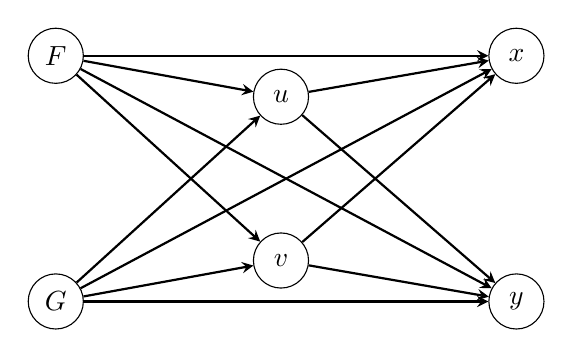
\begin{tikzpicture}[scale=1.3,
    >=stealth,
    var/.style={draw, circle, minimum size=7mm, inner sep=0pt},
    edge/.style={->, thick}]
    
  % 函数 (左)
  \node[var] (F) at (0,1.2)  {$F$};
  \node[var] (G) at (0,-1.2) {$G$};

  % 中间变量 (中，向中间靠拢)
  \node[var] (u) at (2.2,0.8) {$u$};
  \node[var] (v) at (2.2,-0.8){$v$};

  % 自变量 (右)
  \node[var] (x) at (4.5,1.2)  {$x$};
  \node[var] (y) at (4.5,-1.2) {$y$};

  % 函数到中间变量 (F->u, F->v, G->u, G->v)
  \draw[edge] (F) -- (u);
  \draw[edge] (F) -- (v);
  \draw[edge] (G) -- (u);
  \draw[edge] (G) -- (v);

  % 函数直接到自变量 (F->x, F->y, G->x, G->y)
  \draw[edge] (F) -- (x);
  \draw[edge] (F) -- (y);
  \draw[edge] (G) -- (x);
  \draw[edge] (G) -- (y);

  % 中间变量到自变量 (u->x, u->y, v->x, v->y)
  \draw[edge] (u) -- (x);
  \draw[edge] (u) -- (y);
  \draw[edge] (v) -- (x);
  \draw[edge] (v) -- (y);

\end{tikzpicture}
\end{center}

从图中可以看到，$F$ 对 $x$ 的总变化率有三条路径：直接到 $x$，以及经过 $u$ 或 $v$ 再到 $x$。对 $G$ 也是如此。因此链式法则给出：
\[
\begin{cases}
F_x \cdot 1 + F_u \cdot u_x + F_v \cdot v_x = 0\\[4pt]
G_x \cdot 1 + G_u \cdot u_x + G_v \cdot v_x = 0
\end{cases}
\]

把已知的偏导数 $F_x,F_u,F_v$ 和 $G_x,G_u,G_v$ 当作系数，这就是关于未知量 $u_x,v_x$ 的二元一次方程组。解出它，就得到了 $\frac{\partial u}{\partial x}$ 和 $\frac{\partial v}{\partial x}$。

同理，对 $y$ 求偏导可以得到关于 $u_y,v_y$ 的方程组：
\[
\begin{cases}
F_y \cdot 1 + F_u \cdot u_y + F_v \cdot v_y = 0\\[4pt]
G_y \cdot 1 + G_u \cdot u_y + G_v \cdot v_y = 0
\end{cases}
\]

我们以关于未知量 $u_x,v_x$ 的二元一次方程组为例，把$\frac{\partial u}{\partial x}$解出来：

将第一个方程两边同乘 \(G_v\)，第二个方程两边同乘 \(F_v\)：
$$
\begin{cases}
F_u G_v u_x + F_v G_v v_x = -F_x G_v \\
G_u F_v u_x + G_v F_v v_x = -G_x F_v
\end{cases}
$$

两式相减，\(v_x\) 的项消掉，得到：
$$
(F_u G_v - F_v G_u) u_x = -F_x G_v + G_x F_v = F_v G_x - F_x G_v
$$

移项得：
$$
\frac{\partial u}{\partial x} = u_x = \frac{F_v G_x - F_x G_v}{F_u G_v - F_v G_u}
$$

其他偏导数同理。

仔细观察，我们会发现分子分母可以用行列式表示，于是我们有：

\begin{definition}{雅可比行列式}{}
  定义\textbf{雅可比行列式}：
  \[
J = \frac{\partial(F,G)}{\partial(u,v)} =
\begin{vmatrix}
\frac{\partial F}{\partial u} & \frac{\partial F}{\partial v} \\[6pt]
\frac{\partial G}{\partial u} & \frac{\partial G}{\partial v}
\end{vmatrix}
= 
\begin{vmatrix}
F_u & F_v \\
G_u & G_v
\end{vmatrix}
= F_u G_v - F_v G_u
\]

\end{definition}

也就是说，只要 $J \neq 0$，我们就可以写出偏导数的解：
\begin{theorem}{参数方程求偏导公式}{}
  若方程组$\begin{cases}
F(x,y,u,v)=0 \\
G(x,y,u,v)=0
\end{cases}$确定了隐函数$u = u(x,y)$，$v = v(x,y)$，则偏导数为：
\[
\frac{\partial u}{\partial x} = -\frac{\begin{vmatrix}
F_x & F_v \\
G_x & G_v
\end{vmatrix}}{J}
,\qquad
\frac{\partial v}{\partial x} = -\frac{\begin{vmatrix}
F_u & F_x \\
G_u & G_x
\end{vmatrix}}{J}
\]
\[
\frac{\partial u}{\partial y} = -\frac{\begin{vmatrix}
F_y & F_v \\
G_y & G_v
\end{vmatrix}}{J}
,\qquad
\frac{\partial v}{\partial y} = -\frac{\begin{vmatrix}
F_u & F_y \\
G_u & G_y
\end{vmatrix}}{J}
\]
\end{theorem}

观察这些公式，规律其实很清楚，偏导数的分母总是雅可比行列式，分子则是把雅可比行列式的对应列换成 $x$ 或 $y$ 的偏导数列。例如要求$\frac{\partial u}{\partial x}$，$\partial u$在雅可比行列式的第一列，就把第一列所有$\partial u$换成 $\partial x$，其余不变。要求$\frac{\partial v}{\partial y}$，$\partial v$在雅可比行列式的第二列，就把第二列所有$\partial v$换成 $\partial y$，其余不变。

我们来看个例子实践一下：

\begin{myexample}
  设方程组$\begin{cases}
u +\cos v=e^x+\ln y\\
\sin u +v=\ln x+e^y
\end{cases}$确定了隐函数 $u = u(x,y)$，$v = v(x,y)$，求 $\dfrac{\partial u}{\partial x}$ 与 $\dfrac{\partial v}{\partial y}$。

将方程组写成隐函数形式：
\[
\begin{aligned}
F(x,y,u,v) &= u + \cos v - e^x - \ln y = 0 \\
G(x,y,u,v) &= \sin u + v - \ln x - e^y = 0
\end{aligned}
\]

计算一阶偏导数：
\[
\begin{aligned}
F_u &= 1, & F_v &= -\sin v, & F_x &= -e^x, & F_y &= -\frac{1}{y}\\
G_u &= \cos u, & G_v &= 1, & G_x &= -\frac{1}{x}, & G_y &= -e^y
\end{aligned}
\]

关于 $(u,v)$ 的雅可比行列式为：
\[
J = \frac{\partial(F,G)}{\partial(u,v)} =
\begin{vmatrix}
\frac{\partial F}{\partial u} & \frac{\partial F}{\partial v} \\[6pt]
\frac{\partial G}{\partial u} & \frac{\partial G}{\partial v}
\end{vmatrix}
=
\begin{vmatrix}
F_u & F_v \\
G_u & G_v
\end{vmatrix}
= F_u G_v - F_v G_u
= 1\cdot 1 - (-\sin v)\cos u = 1 + \sin v \cos u
\]

要求$\frac{\partial u}{\partial x}$，$\partial u$都在雅可比行列式的第一列，将第一列$\partial u$换为$\partial x$，其余不变，得到：
\[
\frac{\partial u}{\partial x} = -\frac{\begin{vmatrix}
\frac{\partial F}{\partial x} & \frac{\partial F}{\partial v} \\[6pt]
\frac{\partial G}{\partial x} & \frac{\partial G}{\partial v}
\end{vmatrix}}{J} = -\frac{\begin{vmatrix}
F_x & F_v \\
G_x & G_v
\end{vmatrix}}{J}
\]

其中：
\[
\begin{vmatrix}
F_x & F_v \\
G_x & G_v
\end{vmatrix}
= F_xG_v - F_vG_x = (-e^x)\cdot 1 - (-\sin v)(-\frac{1}{x})
= -e^x - \frac{\sin v}{x}
\]

因此：
\[
\frac{\partial u}{\partial x} = -\frac{-e^x - \dfrac{\sin v}{x}}{1 + \sin v \cos u}
= \frac{x e^x + \sin v}{x(1 + \sin v \cos u)}
\]

要求$\frac{\partial v}{\partial y}$，$\partial u$都在雅可比行列式的第二列，将第二列$\partial v$换为$\partial y$，其余不变，得到：
\[
\frac{\partial v}{\partial y} = -\frac{\begin{vmatrix}
\frac{\partial F}{\partial u} & \frac{\partial F}{\partial y} \\[6pt]
\frac{\partial G}{\partial u} & \frac{\partial G}{\partial y}
\end{vmatrix}}{J} = -\frac{\begin{vmatrix}
F_u & F_y \\
G_u & G_y
\end{vmatrix}}{J}
\]

其中：
\[
\begin{vmatrix}
F_u & F_y \\
G_u & G_y
\end{vmatrix}
= F_uG_y - F_yG_u = 1\cdot(-e^y) - (-\frac{1}{y})\cos u
= -e^y + \frac{\cos u}{y}
\]

于是：
\[
\frac{\partial v}{\partial y} = -\frac{-e^y + \dfrac{\cos u}{y}}{1 + \sin v \cos u}
= \frac{y e^y - \cos u}{y(1 + \sin v \cos u)}
\]

综上，
\[
\frac{\partial u}{\partial x} = \frac{x e^x + \sin v}{x(1+\sin v\cos u)},\qquad
\frac{\partial v}{\partial y} = \frac{y e^y - \cos u}{y(1+\sin v\cos u)}
\]

\end{myexample}

看完这个例子，你可能会说这计算量也太大了吧。确实，所以我们还有一招，利用全微分形式不变性，在某种程度上可以更省力地处理这类问题。

我们对两个方程两边同时求全微分：
\[
\begin{cases}
F_x\,dx + F_y\,dy + F_u\,du + F_v\,dv = 0 \\
G_x\,dx + G_y\,dy + G_u\,du + G_v\,dv = 0
\end{cases}
\]

把 $dx,dy$ 看作已知，$du,dv$ 看作未知，这又是一个二元一次方程组。解出 $du,dv$：
\[
du = \frac{\partial u}{\partial x}\,dx + \frac{\partial u}{\partial y}\,dy,\qquad
dv = \frac{\partial v}{\partial x}\,dx + \frac{\partial v}{\partial y}\,dy
\]

也就是说，结果中 $dx$ 的系数就是 $\frac{\partial u}{\partial x}$ 和 $\frac{\partial v}{\partial x}$，$dy$ 的系数就是 $\frac{\partial u}{\partial y}$ 和 $\frac{\partial v}{\partial y}$。这样就求出了所有偏导数。

\begin{theorem}{全微分求偏导数法则}{}
  若方程组$\begin{cases}
F(x,y,u,v)=0 \\
G(x,y,u,v)=0
\end{cases}$确定了隐函数$u = u(x,y)$，$v = v(x,y)$，则：
\[
du = \frac{\partial u}{\partial x}\,dx + \frac{\partial u}{\partial y}\,dy,\qquad
dv = \frac{\partial v}{\partial x}\,dx + \frac{\partial v}{\partial y}\,dy
\]
然后比较系数得到对应偏导数。
\end{theorem}

我们还是以刚刚的例子作示范：

\begin{myexample}
  设方程组$\begin{cases}
u +\cos v=e^x+\ln y\\
\sin u +v=\ln x+e^y
\end{cases}$确定了隐函数 $u = u(x,y)$，$v = v(x,y)$，求 $\dfrac{\partial u}{\partial x}$ 与 $\dfrac{\partial v}{\partial y}$。

对两式两边同时求全微分：
\[
\begin{cases}
du - \sin v\,dv = e^x\,dx + \dfrac{1}{y}\,dy\\[6pt]
\cos u\,du + dv = \dfrac{1}{x}\,dx + e^y\,dy
\end{cases}
\]

先求 $\dfrac{\partial u}{\partial x}$。将第一个方程加上 $\sin v$ 乘以第二个方程，消去 $dv$：

\[
(du - \sin v\,dv) + \sin v(\cos u\,du + dv)
= (e^x\,dx + \frac{1}{y}\,dy) + \sin v(\frac{1}{x}\,dx + e^y\,dy)
\]

左端化简为：
\[
du + \sin v \cos u\,du = (1 + \sin v\cos u)\,du
\]

右端按 $dx,dy$ 合并：
\[
(e^x + \frac{\sin v}{x})\,dx + (\frac{1}{y} + e^y\sin v)\,dy
\]

因此：
\[
du = \frac{e^x + \dfrac{\sin v}{x}}{1 + \sin v\cos u}\,dx
    + \frac{\dfrac{1}{y} + e^y\sin v}{1 + \sin v\cos u}\,dy
\]

由全微分公式 $du = \frac{\partial u}{\partial x}\,dx + \frac{\partial u}{\partial y}\,dy$，即得：
\[
\frac{\partial u}{\partial x} = \frac{e^x + \dfrac{\sin v}{x}}{1 + \sin v\cos u}
      = \frac{x e^x + \sin v}{x(1 + \sin v\cos u)}
\]

再求 $\dfrac{\partial v}{\partial y}$。将第二个方程减去 $\cos u$ 乘以第一个方程，消去 $du$：
\[
(\cos u\,du + dv) - \cos u(du - \sin v\,dv)
= (\frac{1}{x}\,dx + e^y\,dy) - \cos u(e^x\,dx + \frac{1}{y}\,dy)
\]

左端化简为：
\[
dv + \cos u\sin v\,dv = (1 + \sin v\cos u)\,dv
\]

右端按 $dx,dy$ 合并：
\[
(\frac{1}{x} - e^x\cos u)\,dx + (e^y - \frac{\cos u}{y})\,dy
\]

因此：
\[
dv = \frac{\dfrac{1}{x} - e^x\cos u}{1 + \sin v\cos u}\,dx
    + \frac{e^y - \dfrac{\cos u}{y}}{1 + \sin v\cos u}\,dy
\]

由全微分公式 $dv = \frac{\partial v}{\partial x}\,dx + \frac{\partial v}{\partial y}\,dy$，即得：
\[
\frac{\partial v}{\partial y} = \frac{e^y - \dfrac{\cos u}{y}}{1 + \sin v\cos u}
      = \frac{y e^y - \cos u}{y(1 + \sin v\cos u)}
\]

\end{myexample}

对于不同的参数方程，我们可以选取不同的计算方法以简便运算。不过一般而言，这两种方法都差不多，掌握一种就可以求出绝大部分由参数方程确定的隐函数的偏导数了。

\section{方向导数与梯度}
偏导数 $f_x$ 和 $f_y$ 只告诉我们函数沿 $x$ 轴和 $y$ 轴方向的变化率。但实际中我们可能想知道，沿着任意一个方向，函数变化得有多快？比如山坡上某一点，沿正北方向的坡度是多少？沿西北方向呢？这就是我们接下来要讨论的问题。

\subsection{方向导数}
我们想知道，从函数上一点 $P_0$ 出发沿某个方向走一小步 $t$，到达点 $P'_0$，我们关心的是，当这一步越来越小时，函数值的变化是多少？换句话说，如果这一步足够小，是不是可以求得函数在此方向的变化率？由此引出方向导数：

\begin{definition}{方向导数}{}
设 $z = f(x, y)$ 在 $P_0(x_0, y_0)$ 的某个邻域内有定义，$\vec{l} = (\cos\alpha, \cos\beta)$ 是一个单位方向向量。若极限
\[
\lim_{t \to 0^+} \frac{f(x_0 + t\cos\alpha,\; y_0 + t\cos\beta) - f(x_0, y_0)}{t}
\]
存在，则称此极限为 $f$ 在 $P_0$ 处沿方向 $\vec{l}$ 的\textbf{方向导数}，记作 $\dfrac{\partial f}{\partial \vec{l}}\Big|_{P_0}$。
\end{definition}

方向导数就是函数沿某个特定方向的变化率。当 $\vec{l} = (1, 0)$（沿 $x$ 轴正方向）时，方向导数就是 $f_x$，当 $\vec{l} = (0, 1)$（沿 $y$ 轴正方向）时，方向导数就是 $f_y$。所以，偏导数其实是方向导数的特例。

如果函数可微，方向导数有一个非常简洁的计算公式：

\begin{theorem}{方向导数的计算公式}{}
若 $f(x, y)$ 在 $P_0(x_0, y_0)$ 处可微，则沿任意方向 $\vec{l} = (\cos\alpha, \cos\beta)$ 的方向导数为：
\[
\frac{\partial f}{\partial \vec{l}} = f_x(x_0, y_0)\cos\alpha + f_y(x_0, y_0)\cos\beta
\]
\end{theorem}

这个公式说明，只要算出两个偏导数 $f_x$ 和 $f_y$，再乘以方向的分量 $\cos\alpha$ 和 $\cos\beta$，再相加就得到方向导数了。你可能会说，哎呀每次都要算$\cos\alpha$ 和 $\cos\beta$实在是太麻烦了，有没有更简便一点的方法？

其实是有的。刚刚定义里提到，$ (\cos\alpha, \cos\beta)$ 是一个单位方向向量，也就是说，对任意的$\vec{l}$，我们只需要求$\vec{l}$的单位向量就可以了，而$\vec{l}$的单位向量是好求的，我们用$\vec{l}^0$表示$\vec{l}$的单位向量，则$\vec{l}^0=\frac{\vec{l}}{|\vec{l}|}$，这个实际上是高中的数学知识了。

我们来看个例子：

\begin{myexample}
  求 $f(x, y) = x^2 + y^2$ 在点 $(1, 2)$ 处沿方向 $\vec{l} = (1, \sqrt{3})$ 的方向导数。

  先求偏导：$f_x = 2x$，$f_y = 2y$。在 $(1, 2)$ 处，$f_x = 2$，$f_y = 4$。

  方向 $\vec{l} = (1, \sqrt{3})$，则$\vec{l}^0=\frac{\vec{l}}{|\vec{l}|}=(\frac{1}{2},\frac{\sqrt{3}}{2})$。

  代入公式：
  \[
  \frac{\partial f}{\partial \vec{l}} = 2 \cdot \frac{1}{2} + 4 \cdot \frac{\sqrt{3}}{2} = 1 + 2\sqrt{3}
  \]

  结果为正，说明沿这个方向函数值在增加。
\end{myexample}

这就是说，实际计算中，我们并不是一定要求$(\cos\alpha,\cos\beta)$这个向量，绝大多数时候都是求出$\vec{l}^0$，用$\vec{l}^0$代替$(\cos\alpha,\cos\beta)$，因为它们本质上是等价的。

方向导数的几何意义也是好理解的。类比偏导数，方向导数实际上就是函数$z=f(x,y)$沿方向$\vec{l}$的切线斜率。方向导数为正，就说明函数值沿方向$\vec{l}$增加，方向导数为负，就说明函数值沿方向$\vec{l}$减少。

\subsection{梯度及其几何意义}

我们先来仔细观察一下方向导数的公式。我们发现，它可以写成向量的点积形式：
\[
\frac{\partial f}{\partial \vec{l}} = (f_x,\; f_y) \cdot \vec{l}^0=f_x \cos\alpha + f_y \cos\beta
\]

这个公式里面的向量 $(f_x, f_y)$ 表示什么呢？直观上看，这个向量由两个偏导数组成。我们知道，偏导数表示函数对某个自变量的变化率，那么向量 $(f_x, f_y)$表示的是变化率的方向吗？

在此之前，我们先定义Nabla算子：

\begin{definition}{Nabla算子}{}
  定义向量微分算子
\[
\nabla = (\frac{\partial}{\partial x},\; \frac{\partial}{\partial y},\; \frac{\partial}{\partial z})
\]
\end{definition}

这是三维形式的Nabla算子。二维形式也类似，就是去掉$\frac{\partial}{\partial z}$一项。要注意的是，Nabla算子本身不是一个数，你可以把它理解为“$+$”“$-$”这种符号，它是运算符，单独出现时没有意义，一般作用在函数身上，尤其是多元函数。

我们还知道，方向导数是函数$z=f(x,y)$沿方向$\vec{l}$的切线斜率，反映的是函数沿方向$\vec{l}$的变化率，那么，函数沿着哪一个方向变化率最大呢？沿着哪一个方向变化率最小呢？

我们再来观察一下改写之后的方向导数的公式。我们发现，要让方向导数取到最大，$\vec{l}^0$就必须和向量$(f_x, f_y)$同向，因为偏导数由函数决定，而$\vec{l}^0$的方向是可以任取的。当$\vec{l}^0$和向量$(f_x, f_y)$同向时，方向导数正好就等于向量 $(f_x, f_y)$ 的模长，也就是说，向量 $(f_x, f_y)$ 表示的正是方向导数最大的方向，沿着向量 $(f_x, f_y)$ 的函数值变化率最大。同理，当$\vec{l}^0$和向量$(f_x, f_y)$垂直时，点积结果为$0$，此时向量 $\vec{l}^0$ 表示的是方向导数为$0$的方向，沿着向量 $\vec{l}^0$ 的函数值变化率为$0$。那么我们就能够定义：

\begin{definition}{梯度}{}
设 $z = f(x, y)$ 在 $P_0(x_0, y_0)$ 处偏导数存在，则称向量
\[
\nabla f\big|_{P_0} = (f_x(x_0, y_0),\; f_y(x_0, y_0))
\]
为 $f$ 在 $P_0$ 处的\textbf{梯度}。记作 $\nabla f$ 或“grad $f$”。
\end{definition}

梯度的方向决定了函数值变化最快的方向，它的模长决定了函数值变化最快时的速率。\textbf{梯度是个向量}。

引入了Nabla算子，我们可以直接定义梯度的运算。梯度实际上等于Nabla算子与$f$的数乘。
\[
\text{grad} f=\nabla f= (\frac{\partial f}{\partial x},\; \frac{\partial f}{\partial y},\; \frac{\partial f}{\partial z})
\]

当然，这是三维的。二维的写成$(\frac{\partial f}{\partial x},\; \frac{\partial f}{\partial y})$。

有了梯度，我们再来重写方向导数公式：
\[
\frac{\partial f}{\partial \vec{l}}=\nabla f \cdot \vec{l}^0
\]


从这个式子可以立刻看出几件事：

当 $\theta = 0$，即 $\vec{l}$ 与梯度同方向时，方向导数取最大值 $|\nabla f|$，梯度方向是函数值增加最快的方向。

当 $\theta = \pi$，即 $\vec{l}$ 与梯度反方向时，方向导数取最小值 $-|\nabla f|$，沿梯度反方向，函数值减少最快。

当 $\theta = \frac{\pi}{2}$，即 $\vec{l}$ 与梯度垂直时，方向导数为 $0$，沿这个方向，函数值不增不减。

这和我们刚刚讨论的结果是一致的。下图的蓝色箭头表示的是梯度的方向，红色箭头表示的是这个曲面最陡的方向。

\begin{center}
  \begin{tikzpicture}
  \begin{axis}[
      view={55}{10},
      axis lines=none,           % 去掉坐标轴
      domain=-2:2,
      y domain=-2:2,
      samples=35,
      samples y=35,
      colormap/viridis,
  ]
  
  % 曲面 z = 0.2x^2 + 0.1y^2
  \addplot3[
      surf,
      shader=interp,             % 平滑着色，去掉网格线
      opacity=0.65,
  ]
  {0.2*x^2 + 0.1*y^2};
  
  % 点 P = (1,1,f(1,1))
  \addplot3[
      only marks,
      mark=*,
      mark size=1.8pt,
      color=red,
  ]
  coordinates {(1,1,0.3)};
  
  % 梯度向量 (曲面上的上升方向)
  \addplot3[
      ->,
      very thick,
      red,
  ]
  coordinates {
      (1,1,0.3)
      (1.8,1.4,0.7)
  };
  
  \node[red] at (axis cs:1.05,1.85,0.75) {最陡方向};

  \addplot3[
    dashed,
    gray,
    thin,
]
coordinates {
    (1,1,0.3)
    (1,1,0)
};

  \addplot3[
    dashed,
    gray,
    thin,
]
coordinates {
    (1.8,1.4,0.7)
    (1.8,1.4,0)
};

\addplot3[
      only marks,
      mark=*,
      mark size=1.8pt,
      color=blue,
  ]
  coordinates {(1,1,0)};

% 三维向量的水平投影（灰色箭头，在 z=0 平面）
\addplot3[
    ->,
    very thick,
    blue,
]
coordinates {
    (1,1,0)
    (1.8,1.4,0)
};
\node[blue, above] at (axis cs:1.45,1.2,0) {$\nabla f$};
  
  \end{axis}
  \end{tikzpicture}
\end{center}

我们来看个例子：

\begin{myexample}
  求 $f(x, y) = x^2 + y^2$ 在点 $(1, 2)$ 处的梯度，以及函数值增加最快的方向和速率。

  $f_x = 2x$，$f_y = 2y$。在 $(1, 2)$ 处，$\nabla f = (2, 4)$。

  梯度方向 $(2, 4)$ 就是函数值增加最快的方向，增加速率为 $|\nabla f| = \sqrt{4 + 16} = 2\sqrt{5}$。
\end{myexample}

梯度还有一个非常重要的几何意义。设函数$f(x, y)$，平面$z = C$， 那么$f(x, y) = C$就是一条等高线，在等高线上的每一点的梯度 $\nabla f$ 都垂直于等高线。因为沿着等高线走，函数值不变，方向导数为 $0$，即 $\nabla f \cdot \vec{l} = 0$，所以 $\nabla f$ 与等高线的切线方向 $\vec{l}$ 垂直。这和我们之前讲“法向量垂直于平面”的思想完全一致。

想象你在爬山。等高线就是地图上那些闭合的圈。梯度方向就是最陡的上坡方向，它总是垂直于等高线，指向山顶。沿着等高线走，既不上升也不下降。

推广到三元函数 $w = f(x, y, z)$，梯度的定义完全类似，几何上，$\nabla f$ 垂直于等值面 $f(x, y, z) = C$。

\subsection{多元函数微分学的几何应用}

和一元函数类似，导数用来求切线斜率，推广到二元函数，偏导数和全微分就会在切线和切平面上大显身手。

我们先以空间曲线为例。设空间曲线以参数方程$\Gamma: 
\begin{cases}
x = x(t)\\
y = y(t)\\
z = z(t)
\end{cases}$给出，其中 $x(t), y(t), z(t)$ 可导且导数不同时为零。仿照一元函数，我们有：

\begin{theorem}{空间曲线的切向量}{}
若曲线 $\Gamma$ 的参数方程中 $x(t), y(t), z(t)$ 在 $t_0$ 处可导，且导数不全为零，则曲线 $\Gamma$在 $t_0$ 处的切向量为：
\[
\vec{T} = ( x'(t_0),\, y'(t_0),\, z'(t_0) )
\]
\end{theorem}

切向量的几何意义是显然的，当三个方向都取导数时，那么这个向量指向的就是曲线在该点的瞬时方向。也就是说，切向量是曲线在该点的切线的方向向量。已知一点和方向向量，我们就能写出直线：

\begin{theorem}{空间曲线的切线}{}
  若曲线 $\Gamma$ 的参数方程中 $x(t), y(t), z(t)$ 在 $t_0$ 处可导，且导数不全为零，则曲线在 $P_0$ 处的切线方程为：
\[
\frac{x-x_0}{x'(t_0)} = \frac{y-y_0}{y'(t_0)} = \frac{z-z_0}{z'(t_0)}
\]
切向量是切线的一个方向向量。
\end{theorem}

现在有了一点和切向量，我们根据平面的点法式，就能写出一张平面的方程：

\begin{theorem}{法平面}{}
若曲线 $\Gamma$在 $t_0$ 处存在切向量与切线，则曲线 $\Gamma$在 $t_0$ 处的法平面方程为：
\[
x'(t_0)(x-x_0) + y'(t_0)(y-y_0) + z'(t_0)(z-z_0) = 0
\]
法平面过曲线 $\Gamma$ 上一点 $P_0$ 且与该点切线垂直。
\end{theorem}

由于我们把切向量当作平面的法向量，用点法式写出了平面方程，所以切线自然垂直于这个平面。

有了切向量，切线，法平面，我们就能更具体地研究空间曲线了。

\begin{myexample}
求螺旋线 $\Gamma: 
\begin{cases}
x = \cos t\\
y = \sin t\\
z = \frac{t}{10}
\end{cases}$ 在 $t = \frac{\pi}{2}$ 处的切线与法平面方程。

直接对$t$求导，得切向量为 $\vec{T} = (-\sin t,\; \cos t,\; \frac{1}{10})$。在 $t=\frac{\pi}{2}$ 时，$\vec{T} = (-1,0,\frac{1}{10})$。

切线方程：
\[
\frac{x-0}{-1} = \frac{y-1}{0} = \frac{z-\frac{\pi}{20}}{\frac{1}{10}}
\]

这里 $y-1=0$ 一项单独写出，即： 
\[
\begin{cases} x + 10z = \frac{\pi}{2} \\ y = 1 \end{cases}
\]

法平面方程：
\[
-1\cdot(x-0) + 0\cdot(y-1) + \frac{1}{10} \cdot(z-\frac{\pi}{20}) = 0
\]

化简得： $10x - z + \frac{\pi}{20} = 0$。

从图象来看，就是：
\begin{center}
\begin{tikzpicture}[scale=2]
  \tdplotsetmaincoords{55}{135}
  \begin{scope}[tdplot_main_coords]

    % 坐标轴
    \draw[->,thick] (0,0,0) -- (1.5,0,0) node[below left]{$x$};
    \draw[->,thick] (0,0,0) -- (0,1.5,0) node[below right]{$y$};
    \draw[->,thick] (0,0,0) -- (0,0,2.5)   node[above]{$z$};

    % 螺旋线: x=cos(t), y=sin(t), z=t/10
    \draw[
      domain=0:6*pi,
      samples=400,
      smooth,
      variable=\t,
      red,
      thick
    ] plot ({cos(\t r)}, {sin(\t r)}, {\t/10}) node[black, right] {$\Gamma$};

    % 切点 P0 对应 t=π/2
    \coordinate (P0) at (0,1,{pi/20});
    \filldraw[black] (P0) circle[radius=0.8pt] node[above left] {$P_0$};

    % 切向量 T = (-1,0,1/10)，缩放以便观察
    \draw[->, blue, thick] (P0) -- ++({-0.6},0,{0.06}) node[below] {$\vec{T}$};

    % 法平面（半透明矩形）
    % 法向量为 T，两个垂直方向：u=(0,1,0), v=(1,0,10)
    % 验证垂直：u·T=0, v·T=-1+1=0
    % 矩形参数：P0 + a*u + b*v, a∈[-0.5,0.5], b∈[-0.08,0.08]
    \fill[blue!20, opacity=0.5, draw=blue!40, thick]
      ({-0.08}, {1-0.5}, {pi/20 - 0.8}) --
      ({0.08}, {1-0.5}, {pi/20 + 0.8}) --
      ({0.08}, {1+0.5}, {pi/20 + 0.8}) --
      ({-0.08}, {1+0.5}, {pi/20 - 0.8}) -- cycle;

  \end{scope}
\end{tikzpicture}
\end{center}

\end{myexample}

我们知道，空间曲线并不总是由参数方程确定，当空间曲线由两张空间曲面的交线的形式给出时，我们可以借助梯度来求切向量：

\begin{theorem}{曲面交线的切向量}{}
设空间曲线 $\Gamma$ 由方程组
\[
\begin{cases}
F(x,y,z) = 0 \\
G(x,y,z) = 0
\end{cases}
\]
确定，其中 $F,G$ 具有连续偏导数，且在点 $P_0$ 处 $\nabla F(P_0)$ 与 $\nabla G(P_0)$ 不平行，则 $\Gamma$ 在 $P_0$ 处的切向量为：
\[
\vec{T} = \nabla F(P_0) \times \nabla G(P_0)
\]
\end{theorem}

这是因为曲线同时落在两张曲面上，其切向量必须与两张曲面的法向量都垂直，而叉积正好给出这样一个向量。有了切向量，切线方程和法平面方程就能用刚刚的方法写出，此处不再赘述。

我们来看个例子：

\begin{myexample}
求曲线 $\begin{cases} x^2+y^2+z^2=6 \\ x+y+z=0 \end{cases}$ 在点 $(1,1,-2)$ 处的切线。

令 $F=x^2+y^2+z^2-6$，$G=x+y+z$。则：
\[
\nabla F = (2x,2y,2z),\quad \nabla G = (1,1,1)
\]

在 $(1,1,-2)$ 处，$\nabla F = (2,2,-4)$，$\nabla G = (1,1,1)$。因此：
\[
\vec{T} = \nabla F \times \nabla G =
\begin{vmatrix}
\vec{i} & \vec{j} & \vec{k} \\
2 & 2 & -4 \\
1 & 1 & 1
\end{vmatrix}
= (6, -6, 0)
\]

所以切线方程为 $\frac{x-1}{6} = \frac{y-1}{-6} = \frac{z+2}{0}$，或写为 $\begin{cases} x+y=2 \\ z = -2 \end{cases}$的形式。
\end{myexample}

研究完曲线，现在我们更进一步，从曲线转向曲面。先回忆一下梯度的几何意义，其中有一条性质：$\nabla F$ 垂直于等值面。那么，如果现在要求曲面法向量的话，你有没有什么思路呢？是的，我们可以直接用梯度求空间曲面的法向量：

\begin{theorem}{空间曲面的法向量}{}
设曲面 $\Sigma$ 由方程 $F(x,y,z)=0$ 确定，$F$ 在点 $P_0(x_0,y_0,z_0)$ 处可微且 $\nabla F(P_0)\neq \vec{0}$，则曲面在 $P_0$ 处的法向量为
\[
\vec{n} = \nabla F(P_0) = (F_x(P_0), F_y(P_0), F_z(P_0))
\]

特别地，当曲面以函数 $z=f(x,y)$ 形式给出时，令 $F(x,y,z)=f(x,y)-z$，则法向量为：
\[
\vec{n} = (f_x(x_0,y_0),\; f_y(x_0,y_0),\; -1)
\]
\end{theorem}

有了法向量，就说明我们能确定一条直线。显然，这条直线就是空间曲面的法线，直观上看，法向量的方向就是曲面在该点最“直”地离开曲面的方向，也就是法线的方向。

\begin{theorem}{空间曲面的法线}{}
  设曲面 $\Sigma$ 由方程 $F(x,y,z)=0$ 确定，$F$在 $P_0$ 处的法向量为$\vec{n} = \nabla F(P_0) = (F_x(P_0), F_y(P_0), F_z(P_0))$，则法线方程为：
\[
\frac{x-x_0}{F_x(P_0)} = \frac{y-y_0}{F_y(P_0)} = \frac{z-z_0}{F_z(P_0)}
\]

特别地，当曲面以函数 $z=f(x,y)$ 形式给出时，法线方程为：
\[
\frac{x-x_0}{f_x(x_0,y_0)} = \frac{y-y_0}{f_y(x_0,y_0)} = \frac{z-z_0}{-1}
\]
法向量是法线的一个方向向量。
\end{theorem}

现在有了一点和法向量，我们根据平面的点法式，就能写出一张平面的方程：

\begin{theorem}{切平面}{}
  设曲面 $\Sigma$ 由方程 $F(x,y,z)=0$ 确定，$F$在 $P_0$ 处的法向量为$\vec{n} = \nabla F(P_0) = (F_x(P_0), F_y(P_0), F_z(P_0))$，则切平面方程为：
\[
F_x(P_0) \cdot(x-x_0) + F_y(P_0) \cdot(y-y_0) + F_z(P_0) \cdot(z-z_0) = 0
\]

特别地，当曲面以函数 $z=f(x,y)$ 形式给出时，切平面方程为：
\[
z - z_0 = f_x(x_0,y_0)(x-x_0) + f_y(x_0,y_0)(y-y_0)
\]
切平面过曲面$\Sigma$一点$P_0$且与该点法线垂直。
\end{theorem}

要注意的是，切平面虽说是切平面，但是和曲面可能不止一个交点或一条交线。类比一元函数里的切线，有时与曲线的交点可能不止切点一个。

我们比较一下切平面方程与全微分$dz = f_x(x_0,y_0)\,dx + f_y(x_0,y_0)\,dy$就会发现，全微分 $dz$ 恰好是切平面上当自变量从 $(x_0,y_0)$ 变到 $(x_0+dx,y_0+dy)$ 时 $z$ 坐标的增量。这就说明，全微分是曲面在一点处近似的具体表现。也就是说，切平面在局部很好地逼近了曲面，就像切线逼近曲线一样。

\begin{myexample}
求旋转抛物面 $z = x^2 + y^2$ 在点 $(1,1,2)$ 处的切平面与法线方程。

由 $f(x,y) = x^2+y^2$ 可得 $f_x = 2x$，$f_y = 2y$。所以在 $(1,1)$ 处，$f_x=2, f_y=2$。

切平面方程为：
\[
z-2 = 2(x-1) + 2(y-1)
\]

化简得：$2x + 2y - z = 2$。

法线方程为：
\[
\frac{x-1}{2} = \frac{y-1}{2} = \frac{z-2}{-1}
\]
\end{myexample}

本质上，求法线和切平面的思想与一元函数求切线的思想是一脉相承的。

\section{多元函数的极值}
多元函数和一元函数类似，同样可以求极值和最值，不过情况有点不同。我们这里主要以二元函数为例，更多元的函数的研究方法是类似的。

\subsection{无条件极值}

在一元函数中，极值点就是曲线由上升转为下降的“山峰”，或由下降转为上升的“山谷”，在极值点处，切线是水平的，即导数等于零。现在我们要把这个思路搬到二元函数的曲面上。

我们先给出局部极值的精确定义。和一元情形完全类似，“局部”意味着只关心一点附近的小范围。

\begin{definition}{二元函数的极值}{}
设函数 $z = f(x, y)$ 在点 $P_0(x_0, y_0)$ 的某邻域内有定义。

若对该邻域内所有异于 $P_0$ 的点 $(x, y)$，都有：
\[
f(x, y) < f(x_0, y_0)
\]
则称 $f(x_0, y_0)$ 为 $f$ 的一个\textbf{极大值}，$P_0$ 称为\textbf{极大值点}。

若对该邻域内所有异于 $P_0$ 的点 $(x, y)$，都有：
\[
f(x, y) > f(x_0, y_0)
\]
则称 $f(x_0, y_0)$ 为 $f$ 的一个\textbf{极小值}，$P_0$ 称为\textbf{极小值点}。

极大值与极小值统称\textbf{极值}。
\end{definition}

想象一下，如果你站在曲面的一个“山峰”或“谷底”，那么该点的切平面必定是水平的。切平面水平，意味着两个偏导数都是零。这就引出了极值的必要条件。

\begin{theorem}{极值存在的必要条件}{}
若函数 $z = f(x, y)$ 在点 $(x_0, y_0)$ 处具有偏导数，且在该点取得极值，则必有
\[
f_x(x_0, y_0) = 0,\quad f_y(x_0, y_0) = 0
\]
\end{theorem}

我们把满足 $f_x(x_0, y_0)=0$ 且 $f_y(x_0, y_0)=0$ 的点称为\textbf{驻点}。和一元函数一样，驻点不一定是极值点。偏导数不存在的点也可能有极值，不过我们主要讨论可微的函数，这类异常点相对少见。

一个最典型的例子是双曲抛物面，也就是马鞍面。

\begin{myexample}
  求 $f(x, y) = xy$ 的极值。

  先求偏导：$f_x = y$，$f_y = x$。令$f_x=f_y=0$，解得$x=y=0$，所以原点是驻点。

  但它是极值点吗？我们取 $y=x$ 方向，$f(x, x) = x^2 \ge 0$，原点处取极小值 $0$。我们再取 $y=-x$ 方向，$f(x, -x) = -x^2 \le 0$，原点处又取极大值 $0$。
  
  原点一会是极小值，一会是极大值，那么它究竟是不是极值点呢？很遗憾，它并不是。$f(x, y) = xy$ 实际上是没有极值的。
\end{myexample}

这种既非极大也非极小的驻点，或者既是极大也是极小的驻点，我们称为\textbf{鞍点}。直观上看就是这样：

\begin{center}
  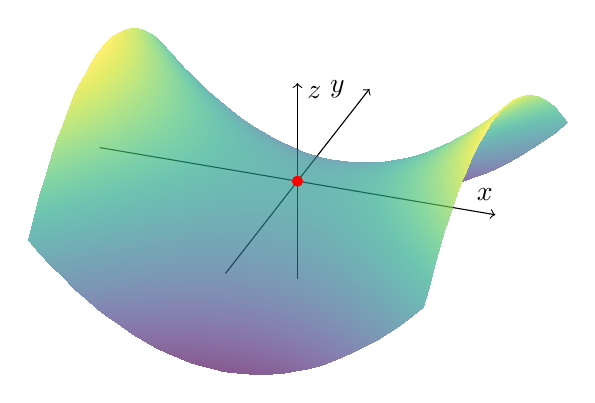
\begin{tikzpicture}
  \begin{axis}[
      view={20}{45},
      axis lines=center,           % 显示穿过原点的坐标轴
      axis line style={->},        % 轴末端带箭头
      xlabel={$x$}, ylabel={$y$}, zlabel={$z$},
      xtick=\empty,
      ytick=\empty,
      ztick=\empty,
      domain=-2.5:2.5,
      y domain=-2.5:2.5,
      samples=35,
      samples y=35,
      colormap/viridis,
  ]
  
  % 马鞍面
  \addplot3[
      surf,
      shader=interp,               % 平滑着色，无网格线
      opacity=0.65,
  ]
  {x^2 - y^2};

  \addplot3[
      only marks,
      mark=*,
      mark size=1.8pt,
      color=red,
  ]
  coordinates {(0,0,0)};
  
  \end{axis}
  \end{tikzpicture}
\end{center}


顾名思义，鞍点就是在马鞍中心的点。那么，如何区分驻点到底是极值点还是鞍点？我们先回忆一下，在一元函数里我们是怎么判断极值点是极大值点还是极小值点的？没错，看二阶导数的正负。二元函数也同样，只不过稍微复杂一点：

\begin{theorem}{极值存在的充分条件}{}
设 $z = f(x, y)$ 在驻点 $P_0(x_0, y_0)$ 的某邻域内具有连续的二阶偏导数。令
\[
A = f_{xx}(P_0),\quad B = f_{xy}(P_0),\quad C = f_{yy}(P_0)
\]
并记判别式 $\Delta = AC - B^2$，则有：

若 $\Delta > 0$，则 $f$ 在 $P_0$ 处取极值，且当 $A > 0$ 时为极小值，当 $A < 0$ 时为极大值。

若 $\Delta < 0$，则 $f$ 在 $P_0$ 处不取极值。

若 $\Delta = 0$，则该方法失效，需用其他办法判断。

\end{theorem}

这个判别法与一元函数的二阶导数判别法本质是一样的。

我们来看一个例子：

\begin{myexample}
  求函数 $f(x, y) = x^3 + y^3 - 3xy$ 的极值。

  首先求偏导，令偏导等于零，解方程组：
  \[
  \begin{cases}
    f_x = 3x^2 - 3y = 0\\
    f_y = 3y^2 - 3x = 0
  \end{cases}
  \]

  解得 $\begin{cases}
    y = x^2\\
    x = y^2
  \end{cases}$，代入得 $x = x^4$，即 $x(x^3 - 1) = 0$。解得两个驻点：$(0, 0)$ 和 $(1, 1)$。

计算二阶偏导数：
  \[
  f_{xx} = 6x,\quad f_{xy} = -3,\quad f_{yy} = 6y
  \]

逐点判别：

在 $(0, 0)$ 处：$A = 0$，$B = -3$，$C = 0$，$\Delta = 0\cdot0 - (-3)^2 = -9 < 0$。判别式小于零，所以 $(0, 0)$ 不是极值点。

在 $(1, 1)$ 处：$A = 6$，$B = -3$，$C = 6$，$\Delta = 6\cdot6 - (-3)^2 = 36-9=27 > 0$。又 $A=6>0$，所以 $f$ 在 $(1, 1)$ 处取得极小值，极小值为 $f(1, 1) = 1+1-3 = -1$。

\end{myexample}

总结一下找无条件极值的基本流程：

先求两个偏导数，找出所有驻点，然后用二阶判别法逐一检验。

\subsection{条件极值}

无条件极值是在定义域内部自由地找最大值最小值。但实际中常常有附加的约束条件。例如在周长固定的矩形中，什么时候面积最大？这时候自变量 $(x, y)$ 不能在整个定义域上随便取，而必须满足某个方程 $g(x, y) = 0$。这种带约束的极值问题，叫做\textbf{条件极值}。

最直接的想法是，从约束方程 $g(x, y) = 0$ 中解出一个变量，代入 $f(x, y)$，化为一元函数的无条件极值。比如约束是 $y = 2x$，直接代入 $f(x, 2x)$ 变成 $x$ 的一元函数就行。但如果约束方程很复杂，解不出 $y$ 关于 $x$ 的显式表达式。这时候要怎么办呢？

拉格朗日在他1788年的巨著《分析力学》中介绍了一个方法：

\begin{definition}{拉格朗日乘数法}{}
  设目标函数$f(x, y)$和$m$个约束函数$g_k(x, y)=0 \ (k=1,2,\dots,m)$均连续可微，构造\textbf{拉格朗日函数}：
  \[
  \mathcal{L}(x, y, \lambda_1, \lambda_2, \dots, \lambda_m)=f(x, y) +\sum_{k=1}^{m} \lambda_k g_k(x, y)
  \]
  其中$\lambda_1, \lambda_2, \dots, \lambda_m$称为\textbf{拉格朗日乘数}。

  若点$P(x_0,y_0)$是目标函数$f(x, y)$在约束$g_k(x, y)=0$下的极值点，则必然存在一组拉格朗日乘数$\lambda_1, \lambda_2, \dots, \lambda_m$，
  使得：
  \[
    \frac{\partial \mathcal{L}}{\partial x}=0, \quad
    \frac{\partial \mathcal{L}}{\partial y}=0, \quad
    \frac{\partial \mathcal{L}}{\partial \lambda_1}=0, \quad
    \frac{\partial \mathcal{L}}{\partial \lambda_2}=0, \quad
    \dots, \quad
    \frac{\partial \mathcal{L}}{\partial \lambda_m}=0
  \]
\end{definition}

拉格朗日乘数法的核心思想是构造一个新的辅助函数，然后对这个多变量函数求无条件极值。令拉格朗日函数对所有变量的偏导数全为零，解这个方程组，得到的解就是可能的条件极值点。也就是说，拉格朗日乘数法的巧妙之处在于把约束条件“吞”进了辅助函数的偏导数为零的条件里，把条件极值转换为了无条件极值。

为什么这样做是对的？我们从几何上看，约束 $g(x, y) = 0$ 是平面上的一条曲线。$f(x, y)$ 在这条曲线上取极值时，$f$ 的梯度 $\nabla f$ 和约束曲线的法向量 $\nabla g$ 必须是平行的，因为如果它们不平行，沿着曲线走一小步，$f$ 的值就会变化。因此极值点处 $\nabla f = -\lambda\, \nabla g$，而这正是$\frac{\partial \mathcal{L}}{\partial x}=0$和
    $\frac{\partial \mathcal{L}}{\partial y}=0$的含义。

我们来看开头的那个例子：

\begin{myexample}
  求周长为定值 $L$ 的矩形中面积的最大值。

  设矩形的长为 $x$、宽为 $y$，则面积 $S = xy$。周长约束为 $2x + 2y = L$，即 $x + y = \frac{L}{2}$。

  构造拉格朗日函数：
  \[
  \mathcal{L}(x, y, \lambda) = xy + \lambda (x + y - \frac{L}{2})
  \]

  求偏导：
  \[
  \frac{\partial \mathcal{L}}{\partial x} = y + \lambda = 0,\quad
  \frac{\partial \mathcal{L}}{\partial y} = x + \lambda = 0,\quad
  \frac{\partial \mathcal{L}}{\partial \lambda} = x + y - \frac{L}{2} = 0
  \]

  前两个方程得 $y = -\lambda$，$x = -\lambda$，即 $x = y$。

  代入约束，$2x = \frac{L}{2}$，得 $x = y = \frac{L}{4}$。此时面积最大，为 $S = \frac{L^2}{16}$。

\end{myexample}

  因此，在周长固定的矩形中，正方形面积最大。

\begin{myexample}
  求 $f(x, y) = x^2 + y^2$ 在约束 $x + y = 1$ 下的极值。

  约束方程写成 $g(x, y) = x + y - 1 = 0$。构造拉格朗日函数：
  \[
  \mathcal{L}(x, y, \lambda) = x^2 + y^2 + \lambda(x + y - 1)
  \]

  求偏导并令其为零：
  \[
  \frac{\partial \mathcal{L}}{\partial x} = 2x + \lambda = 0,\quad
  \frac{\partial \mathcal{L}}{\partial y} = 2y + \lambda = 0,\quad
  \frac{\partial \mathcal{L}}{\partial \lambda} = x + y - 1 = 0
  \]

  前两个方程得 $x = -\frac{\lambda}{2}$，$y = -\frac{\lambda}{2}$，即 $x = y$。
  
  代入第三个方程：$x + x = 1$，得 $x = y = \frac{1}{2}$，$\lambda = -1$。

  因此极值为 $f(\frac{1}{2}, \frac{1}{2}) = \frac{1}{2}$。
  
  几何上，这表示原点 $(0, 0)$ 到直线 $x + y = 1$ 的最短距离的平方。
\end{myexample}

拉格朗日乘数法可以推广到多个变量和多个约束的情形。不过我们主要讨论二元函数带一个约束。

我们用拉格朗日乘数法找到的极值点通常要进一步判断是极大值还是极小值。但在很多实际应用中，问题的背景已经暗示了是极大值还是极小值，即使不做严格判定，依据实际背景也能得到正确答案。

最后我们给一道不等式的题目。也许你高中的时候可能会觉得这种题目很难，但现在有了拉格朗日乘数法这个工具，你不妨用它来算一算。

\begin{myexample}
  已知非负实数 \(a, b, c\) 满足\(a + b + c = 1\)，求 \(a^3 + b^3 + c^3 + 6abc\) 的最大值。

我们在这里只给出不等式的解法。拉格朗日乘数法留给读者。

由$(a+b+c)^3 = a^3+b^3+c^3 + 3(a+b)(b+c)(c+a)$，代入 \(a+b+c=1\)，原式化为：

\[
a^3+b^3+c^3+6abc = 1 - 3(a+b)(b+c)(c+a) + 6abc
\]

由均值不等式，对非负实数有：$a+b \ge 2\sqrt{ab}$，$b+c \ge 2\sqrt{bc}$，$c+a \ge 2\sqrt{ca}$，相乘得：
\[
(a+b)(b+c)(c+a) \ge 8abc
\]

代入得：
\[
1 - 3(a+b)(b+c)(c+a) + 6abc \le 1 - 3 \cdot 8abc + 6abc = 1 - 18abc \le 1
\]

当且仅当\(a,b,c\) 中有两个为 \(0\)，另一个为\(1\)时两个等号同时成立。
\end{myexample}


